%Balíčky
\documentclass[a4paper,11pt,twoside]{article}
\usepackage[utf8]{inputenc} %kodovani, abychom mohli jednoduse psat diakriticka pismena
\usepackage[czech]{babel}
\usepackage{pifont}
\usepackage{graphicx} %pro vkladani obrazku
\usepackage{color}
\usepackage{fancyhdr} %zahlavi a zapati
\usepackage{ifpdf}
\usepackage{amssymb}
\usepackage{booktabs}
\usepackage{subfigure}
\usepackage{titlesec}
\usepackage[multiple]{footmisc}
\usepackage[final]{pdfpages}    % pro vkládání PDF souborů
\usepackage{pdflscape}   % pro sazbu stránek naležato
\usepackage{color}       % pro zvýraznění textu barvou
\usepackage{multirow} 
\usepackage{amsmath}
\usepackage{sectsty}
\usepackage[justification=centering]{caption}
\usepackage[top=1.5cm, left=3cm, right=3cm, bottom=2cm, headheight=26pt, includeheadfoot]{geometry}
\usepackage[colorlinks=false,urlcolor=black]{hyperref}
\usepackage{xcolor}
\usepackage{listings}
\hypersetup{
    colorlinks=true,
    linkcolor=black,
    filecolor=black,      
    urlcolor=black,
    citecolor=black
}
\allsectionsfont{\rmfamily} 

\sectionfont{\huge}
\subsectionfont{\LARGE}
\subsubsectionfont{\Large}

\def\author{Autoři: Bc. Linda Kladivová, Bc. Jana Špererová}
\def\nazevprace{MNOŽINOVÉ OPERACE S POLYGONY}

\begin{document}
\setcounter{page}{1}  % nastaví čítač stránek od stránky Úvod na stránku č. 7
\sloppy
\setlength{\parskip}{1pt}


%%  ÚVODNÍ STRÁNKA %%%%%%%%%%%%%%%%%%%%%%%%%%%%%%%%%%%%%%%%%%%%%%

\pagestyle{empty} % vypne číslování stránek na úvodní straně

\begin{center}
\renewcommand{\baselinestretch}{1.4} %zvetseni mezery mezi radky

\LARGE
\textsc{České vysoké učení technické v~Praze} \\
\textsc{Fakulta stavební} \\

\bigskip

\large
\textsc{PROGRAM GEODÉZIE A KARTOGRAFIE} \\
\textsc{OBOR GEOMATIKA} \\

\vspace{10ex}

\begin{figure}[hbt!] %vlozeni loga
\begin{center}

\includegraphics[width=7cm]{pictures/symbol_cvut_konturova_verze_cb.pdf} 
\end{center}
\end{figure}

\vspace{20ex}

\large
\textsc{\nazevprace} \\
\smallskip


\vspace{6ex}

\normalsize
\textsc{\author} \\
\bigskip
\normalsize
\textsc{Předmět: Algoritmy digitální kartografie a GIS} \\

\end{center}


%% 2. STRÁNKA OBSAHUJE ZADÁNÍ
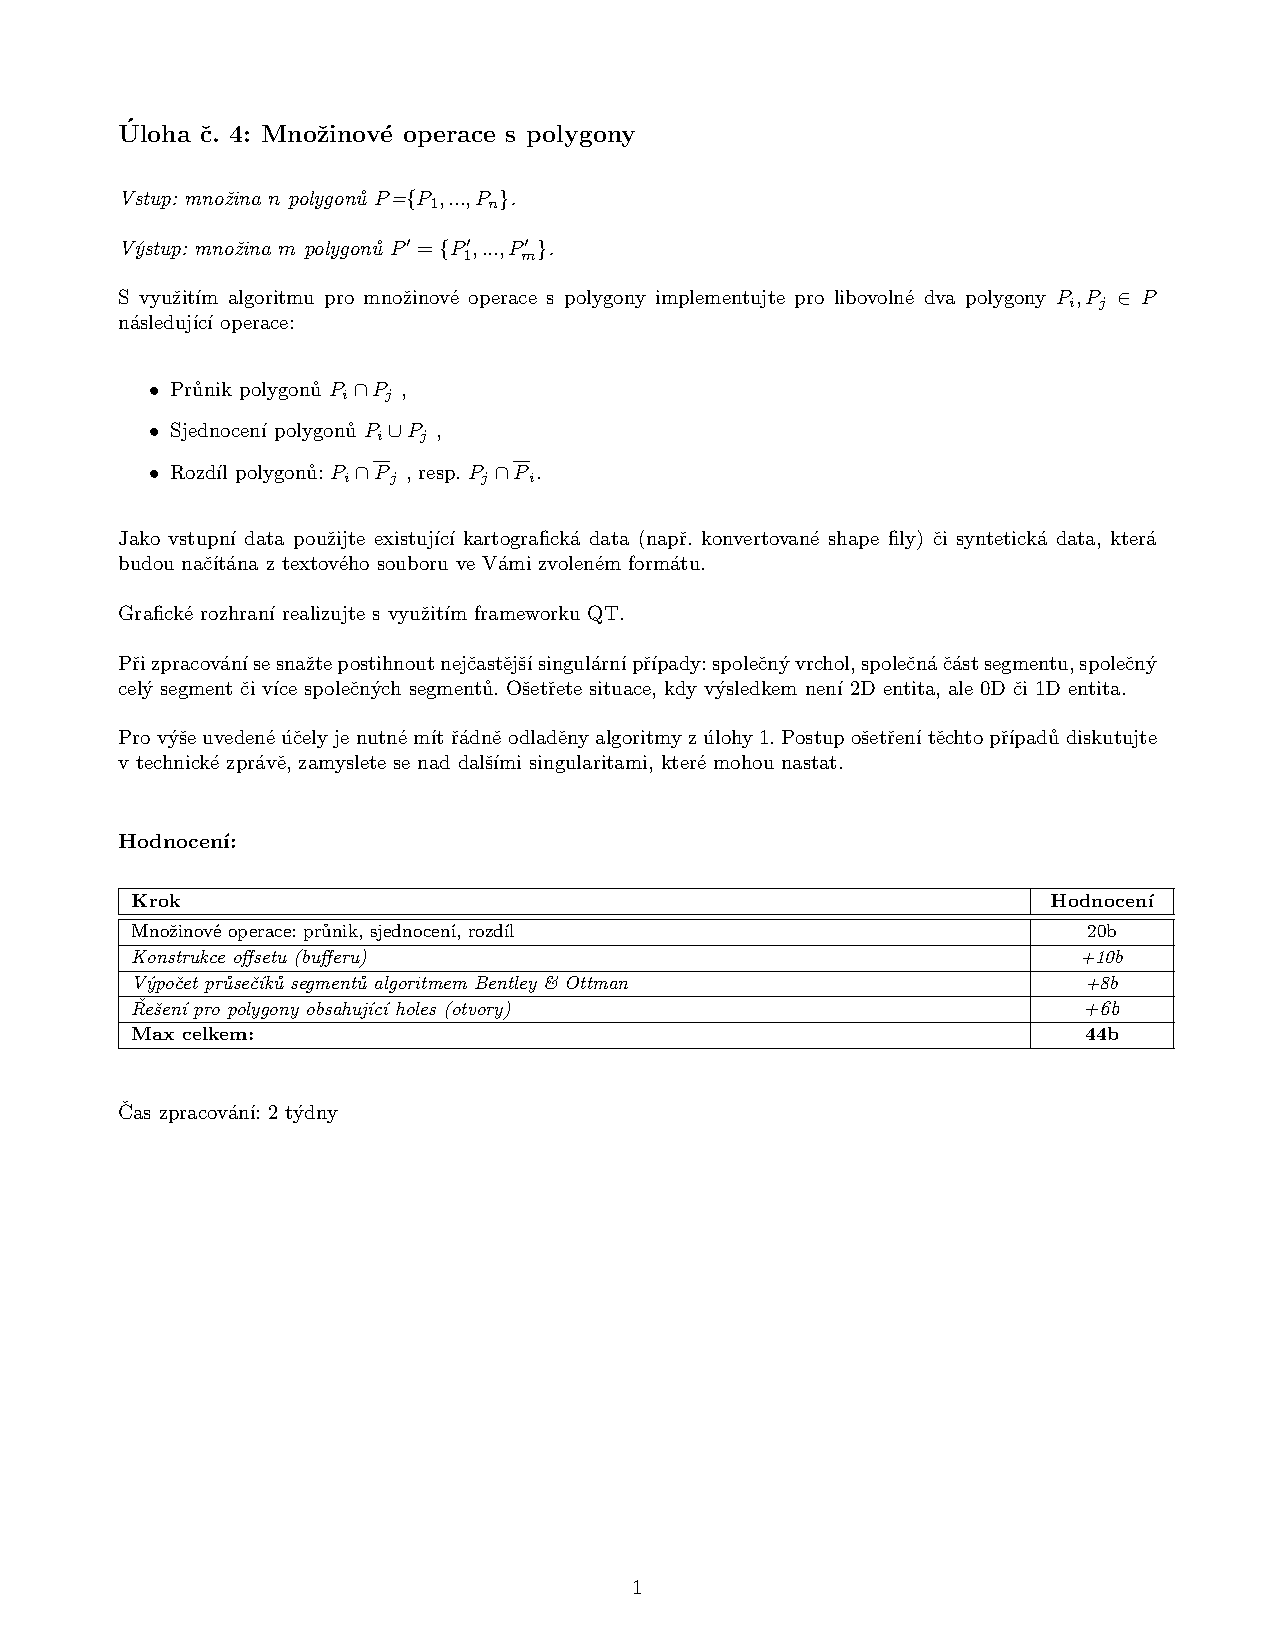
\includepdf{pictures/adkcv4}


%% 3. a 4. STRÁNKA = OBSAH A SEZNAM OBRAZKU %%%%%%%%%%%%%%%%%%%%%%%%%%%%%%%%%%
\renewcommand{\baselinestretch}{1.4} %zvetseni mezery mezi radky
\newpage
\tableofcontents %obsah

\newpage
\listoffigures %seznam obrázků
%\listoftables %seznam tabulek

\thispagestyle{empty}
\newcommand{\obrazek}[1]{(viz obr. \ref{#1})} %specialni reference na obrazek

\newpage
\pagestyle{fancy}

%% NASTAVENI VZHLEDU STRANEK (ZAHLAVI A ZAPATI)

% zajistí, že se názvy kapitol a sekcí nebudou sázet velkými písmeny
\renewcommand{\sectionmark}[1]{\markright{\ #1}}

\fancyhf{} % smaže aktuální nastavení záhlaví a zápatí
\renewcommand{\headrulewidth}{0.4pt} % vrchní linka
\renewcommand{\footrulewidth}{0.4pt}  %  spodní linka
\addtolength{\voffset}{-0.4cm}

 %záhlaví
\fancyhead[LE, LO]{{
\includegraphics[width=1cm]{pictures/symbol_cvut_konturova_verze_cb.pdf} }
   {\textsc{\small {ČVUT v Praze}} }} %logo skoly
\fancyhead[RE, RO]{\nouppercase{\rightmark}}
   
 %zápatí
\fancyfoot[RO, LE]{{\textsc{\small \thepage}}}

\fancypagestyle{plain}{
  \fancyhead{} % na prázdných stránkách nechci záhlaví
  \renewcommand{\headrulewidth}{0pt} % ani linku
}


%% -------<<< 1. KAPITOLKA = Popis a rozbor problému >>>-------\\%%

\pagestyle{fancy}
\fancyhead[RE, RO]{\fancyplain{}{\small \sl{POPIS A ROZBOR PROBLÉMU}}}
\newpage

\vspace*{-1cm}
\section{Popis a rozbor problému}
\large
\renewcommand{\baselinestretch}{1.4}
\noindent Hlavním cílem této úlohy je vytvoření aplikace, která bude umět provádět z vygenerovaných polygonů základní matematické operace – sjednocení, rozdíl a průnik, viz obrázek \ref{fig:operace}.\\
\indent Tyto operace mají velké využití a to nejen v matematice. Používáme je například v GIS, v kartografii a ve spoustě dalších odvětví. Vyskytují se všude kolem nás. Pro určení vztahů těchto operací můžeme použít Booleovské operátory, kdy datové typy mají pouze dvě hodnoty, buď TRUE nebo FALSE. Tedy máme průnik (AND), kdy platí všechna kritéria zároveň, máme sjednocení (OR), kdy platí jedno nebo druhé kritérium nebo poté máme negaci (NOT) a tedy, že něco neplatí.

\vspace{0.2cm}
\begin{figure}[hbt!] 
\begin{center}
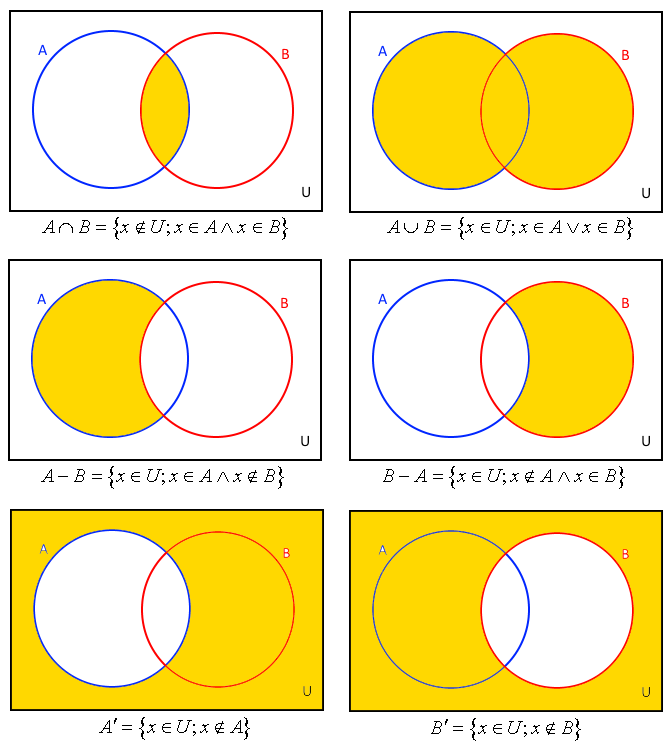
\includegraphics[width=12cm]{pictures/operace.png} 
\caption[Matematické operace - průnik, sjednocení, rozdíl \cite{problem2}]{Matematické operace - průnik, sjednocení, rozdíl, doplněk \cite{problem2}}
\label{fig:operace}
\end{center}
\end{figure}

\noindent\textbf{Sjednocení}\\
\noindent Sjednocení je množinová operace, jejímž výstupem je oblast vyplněná všemi daty z množiny A a zároveň i všemi daty z množiny B. Čili, všechna data z obou množin spadají do požadovaného výsledku.\\

\noindent\textbf{Průnik}\\
\noindent Průnik je množinová operace, kde výstupem je pouze ta oblast, která obsahuje data, která spadají jak do množiny A, tak zároveň i do množiny B. Jinými slovy, výstupem je pouze ta část, kterou obě množiny mají společnou.\\

\noindent\textbf{Rozdíl}\\
\noindent Rozdíl je množinová operace, která má na výstupu oblast množiny, od které „odečítáme“ druhou množinu, avšak bez oblasti průniku těchto dvou množin. Jinak řečeno, od sjednocení těchto dvou množin odebereme celou jednu množinu.\\

Při bližším zkoumání výše jmenovaných matematických operací, je zřejmé, že existují singulární situace. Výsledkem operací může být  linie, polygon, nebo také entita dimenze 0 (bod). Existují následující singulární situace, viz obrázek \ref{fig:problem}: 

\begin{enumerate}
\item Jeden společný vrchol [A]
\item Vrchol leží na hraně druhého polygonu [B]
\item Více společných vrcholů [C]
\item Společná hrana [D]
\item Společná část hrany [E]
\item Hrana leží v hraně druhého polygonu [F]
\end{enumerate}

\vspace{0.2cm}
\begin{figure}[hbt!] 
\begin{center}
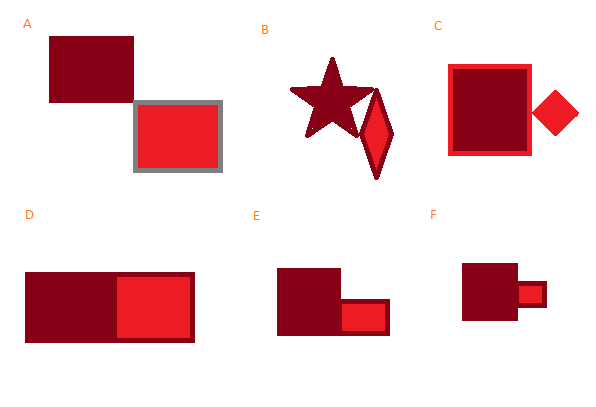
\includegraphics[width=13cm]{pictures/problem.PNG} 
\caption[Problematické situace u množinových operací]{Problematické situace u množinových operací}
\label{fig:problem}
\end{center}
\end{figure}

\noindent Při variantách A, B (tedy 1 nebo více společných vrcholů) bude výsledkem operace INTERSECT prázdná množina, jelikož typ výsledku našich operací je vektor hran. Nicméně reálně by průnikem měl být jeden nebo více společných bodů. Při operaci UNION dojde ve všech případech ke sjednocení obou polygonů, v tomto případě součtu vínového a růžového polygonu. Pokud by měly polygony společný vrchol/vrcholy na hraně, tak výsledkem operace UNION bude znovu součet vínového a růžového polygonu. Průnik bude znovu pouze v bodě, v naší aplikaci není průnik pouze v bodě řešen. \\
\indent V případě variant C. D a E je výsledkem oprace INTERSECTION linie. Do sjednocení tato společná hrana nepatří. Polygon, který by měl vrchol větší než stupeň dva, by byl nekorektní. Výsledek operace DIFFERENCE výše zmíněných situací by měl být jeden ze vstupních polygonů.

\subsection{Údaje o bonusových úlohách}
\large
V rámci úlohy nebyly řešeny žádné bonusové úlohy.

%% -------<<< 2. KAPITOLKA = Popis a rozbor použitých algoritmů >>>-------\\%%

\newpage
\vspace*{-1cm}
\renewcommand{\baselinestretch}{1.4} %zvetseni mezery mezi radky
\pagestyle{fancy}
\fancyhead[RE, RO]{\fancyplain{}{\small \sl{POPIS POUŽITÝCH ALGORITMŮ}}}
\section{Popis použitých algoritmů}
Pro nakreslenou nebo naimportovanou dvojici polygonů chceme určit výsledek množinových operací. Pro tvorbu této aplikace bylo použito několik dílčích algoritmů. Výsledkem tohoto postupu jsou dílčí oblasti, na něž je pak relativně snadné aplikovat množinové operace. \\
\indent Základem bylo vytvoření nového datového typu QPointFB, který si nese informace o parametrech $\alpha$ a $\beta$, které popisují, zda se jedná o průsečík, a dále si nese informaci o poloze bodu vůči polygonu. \\
\indent Aby byla celá práce přehlednější, byla založena třída \textit{types}, do které byly nadefinovány typy, jež jsou pak speciálně použity jako návratové typy různých funkcí. Jedná se o výčtové typy TPointLinePosition (LeftHp = 0, RightHp = 1, Colinear = 2), TPointPolygonPosition (Inner, Outer, On), TBooleanOperation (Union, Intersect, DifferenceAB, DifferenceBA) a T2LinePosition (Parallel, Identical, NonIntersected, Intersected). Tyto typy jsou použity ve funkcích, které byly vytvořeny pro různé fáze algoritmu.\\

\noindent Soupis dílčích fází algoritmu pro určení výsledku různých množinových operací:
\begin{enumerate}
\item Výpočet průsečíků obou polygonů A, B
\item Vsunutí průsečíků do polygonů A, B
\item Ohodnocení vrcholů polygonů A resp. B dle pozice vůči B resp. A
\item Výběr hran podle pozice
\item Sestavení hran pro zadanou množinovou operaci
\end{enumerate}

\noindent Jednotlivé dílčí algoritmy jsou dále podrobně rozebrány.

\newpage
\vspace*{-1cm}
\subsection{Výpočet průsečíků obou polygonů A, B}
\noindent Výpočet průsečíků obou polygonů A, B + setřídění
V tomto algoritmů se prochází body obou polygonů a pomocí funkce get2LinesPosition se hledá zda se vytvořené úsečky z daného a následujícího bodu protínají. K tomuto účelu je na začátku vytvořena proměnná typu Map (slovník). Pokud je nalezen průsečík, je uložen spolu s hodnotu alfa do slovníku. Tento bod je uložen do příslušného polygonu na příslušné místo (dovnitř polygonu) pomocí funkce  ProcessIntersection. Obdobně jsou zpracovány průsečíky u polygonu A.

\subsubsection{Slovní zápis algoritmu}
\begin{enumerate}
\item Pro všechna i: $for (i = 0; i < n; i++)$
\item Vytvoření mapy: $ M = map<double, QPointFB>$
\item Pro všechna j: $for (j = 0; j < m; j++)$
\subitem Pokud existuje průsečík: $if (b_{ij} = (p_i, p_{(i+1)\%n}) \cap (q_j, q_{(j+1)\%m})  \neq \emptyset  )$
\subitem Přidání do mapy: $M[\alpha_i] \leftarrow b_{ij}$
\subitem Zpracování prvního průsečíku: $ProcessIntersection (b_{ij}, \beta, B, j)$
\item Při nalezení průsečíků: $if (\| M \| > 0) $
\subitem Procházení všech průsečíků: $for \forall m \in M$
\subitem Zpracování aktuálního průsečíku: $ProcessIntersection(b, \alpha, A, i)$
\end{enumerate}

\subsection{Vsunutí průsečíků do polygonů A, B}
Do metody ProcessIntersection vstupuje bod, který je průsečíkem, koeficient přímky alfa nebo beta označen t, polygon a index pořadí počátečního bodu úsečky, na které leží průsečík.

\subsubsection{Slovní zápis algoritmu}
\begin{enumerate}
\item Pokud se koeficient t blíží nule. $ if( abs(t) < eps )$
\subitem Vlož průsečík za počáteční bod úsečky
\end{enumerate}

\newpage
\vspace*{-1cm}
\subsection{Ohodnocení vrcholů polygonů A resp. B dle pozice vůči B resp. A}
Počítá už s polygony, do kterých byly vloženy průsečíky. Metoda setPositions prochází prvně zadaný polygon a počítá středový bod daného bodu a následujícího (střed úsečky). Dále určí pozici druhotně zadaného polygonu a středu úsečky pomocí funkce positionPointPolygonWinding. Ke každému procházenému bodu nastaví pozici (Inner, Outer, On). 

\subsubsection{Slovní zápis algoritmu}
\begin{enumerate}
\item Pro všechny body polygonu A. $ for( all points in polygon A ) $
\subitem Vypočti střed hrany polygonu. $ x/y = (poly[i] + poly[i+1])/2 $
\subitem Zjisti pozici středu oproti polygonu B . $ positionPointPolygonWinding() $
\subitem Nastav pozici počátečnímu bodu hrany . $ setPosition = INNER/OUTER/ON $
\item Pro všechny body polygonu B. $ for( all points in polygon B ) $
\subitem Vypočti střed hrany polygonu. $ x/y = (poly[i] + poly[i+1])/2 $
\subitem Zjisti pozici středu oproti polygonu A . $ positionPointPolygonWinding() $
\subitem Nastav pozici počátečnímu bodu hrany . $  setPosition = INNER/OUTER/ON $
\end{enumerate}

\subsection{Výběr hran podle pozice}
V této části jsou vybírány hrany, které mají vůči zadanému polygonu určitou pozici. Pokud má bod v polygonu zadanou pozici vůči polygonu je sestavena hrana. 

\subsubsection{Slovní zápis algoritmu}
\begin{enumerate}
\item Pro všechny body polygonu. $ for( all points in polygon A ) $
\subitem Pokud se pozice bodu rovná zadané pozici (INNER, OUTER, ON), vytvoř hranu.
\end{enumerate}

\newpage
\vspace*{-1cm}
\subsection{Sestavení hran pro zadanou operaci}
Pokud je vybrána operace UNION, jsou vybrány vnější hrany k polygonu A (OUTER) a vnější hrany z polygonu B.
Pokud je vybrána operace INTERSECT, jsou vybrány vnitřní hrany k polygonu A (INNER) a vnitřní hrany z polygonu B.
Pokud je vybrána operace DIFFERENCEAB, jsou vybrány vnější hrany k polygonu A a vnitřní hrany z polygonu B a kolineární segmenty polygonu A.
Pokud je vybrána operace DIFFERENCEBA, jsou vybrány vnější hrany k polygonu B a vnitřní hrany z polygonu A a kolineární segmenty polygonu B.

\subsubsection{Problematické situace a jejich rozbor}
Pokud je středový bod přímo na hraně polygonu, tedy nelze rozhodnout, zda je bod uvnitř nebo mimo polygon, je pozice bodu ON. To samé platí pro hrany. Pozice hrany, která není uvnitř ani mimo polygon, je rovněž ON. V obou těchto zmíněných případů jsou výsledkem operací průnik a sjednocení méně než tři segmenty. Pokud je výstupem množina definovaná méně než třemi segmenty, výstupem je potom prázdná množina. \\
\indent U případů D, E, F u operací průnik i sjednocení nebyly tedy zahrnuty kolineární segmenty. Důležité je si uvědomit, že tyto kolineární hrany se nenacházejí uvnitř množiny, ale pouze na její hranici. U operace union byly zahrnuty pouze vnější segmenty, zatímco u operace intersect pouze ty vnitřní. \\
\indent U průsečíků A, B, C, kde se nachází kolineární segment v podobě jednoho nebo více bodů rovněž nebyly kolineární segmenty uvažovány. U operací rozdíl kolineární segmenty zahrnuty byly, a to u operace A-B kolineární segment k polygonu A, a u operace B-A kolineární segment k polygonu B. 

\newpage
\vspace*{-1cm}
\subsection{Winding Number Algorithm}
\large
\noindent Tento algoritmus byl využit ve funkci setPosition při zjišťování pozice středu úsečky polygonu A vůči polygonu B a naopak.
\\
\noindent Tento algoritmus je také nazýván Metoda ovíjení. Půjdeme postupně po vrcholech polygonu P a budeme sčítat nebo odečítat úhly mezi daným bodem q a vrcholy P (po směru hodinových ručiček přičítáme, proti směru odečítáme). Pokud je výsledný úhel roven 2$\pi$, byl dokončen celý kruh, lze tedy prohlásit, že bod q náleží polygonu P. Pokud je výsledný úhel roven 0, bod q polygonu P nenáleží. Princip Winding algoritmu je zřejmý z obrázku. Při této mětodě byla uvažována malá tolerance, jelikož je pravděpodobné, že výsledný úhel není roven přesně 2$\pi$ nebo 0.

\noindent Při této metodě je zapotřebí počítat Winding Number $\Omega$. Pro toto číslo platí, že je rovno sumě všech rotací $\omega$ proti směru hodinových ručiček, které průvodič opíše nad všemi body: 
$$ 
\Omega = \frac{1}{2\pi} \sum_{i=1}^n \omega_i
$$.

\noindent Platí, že pokud je úhel $\sphericalangle p_i, q, p_{i+1}$ orientován ve směru hodinových ručiček, pak $\omega_i > 0$.
Naopak pokud je úhel $\sphericalangle p_i, q, p_{i+1}$ orientován proti směru hodinových ručiček, pak $\omega_i < 0$.
V závislosti na výsledné hodnotě $\Omega$ lze rozhodnout o poloze bodu q vůči polygonu P:

\begin{itemize}
\item pokud je $\Omega = 1$, platí $q \in P$, 
\item pokud je $\Omega = 0$, pak platí $q { \not \in } P$.
\end{itemize}

\subsubsection{Slovní zápis algoritmu}
\begin{enumerate}
\item Nastavení výchozího úhlu $\omega = 0$ , volba tolerance $\epsilon = 1e-6$.
\item Určení úhlu: $\omega_i = \sphericalangle p_i, q, p_{i+1}$.
\item Určení orientace $o_i$ bodu q ke straně $p_i, p_{i+1}$.
\item Volba podmínky - pokud bod vlevo: $\omega = \omega + \omega_i$, v opačném případě: $\omega = \omega - \omega_i$.
\item Volba podmínky - pokud rozdíl: $|(|\omega| - 2\pi)| < \epsilon$, pak platí: $q \in P$, v opačném případě:  $ q { \not \in } P $.
\end{enumerate}

\subsubsection{Výsledný algoritmus}
Po vytvoření zmíněných dílčích algoritmů jsou funkce postupně volány ve funkci booleanOperations:
\begin{enumerate}
\item Výpočet průsečíků A, B: $ComputeIntersections(A, B)$
\item Určení polohy vrcholů vůči oblastem: $setPosition(A, B) $
\item Určení polohy vrcholů vůči oblastem: $setPosition(B, A) $
\item Výběr hran podle zadané operace $selectEdges(polygon, position, result)$
\end{enumerate}

%% -------<<< 3. KAPITOLA = Vstupní  data >>>-------\\%%
\newpage
\fancyhead[RE, RO]{\fancyplain{}{\small \sl{VSTUPNÍ A VÝSTUPNÍ DATA}}}

\vspace*{-1cm}
\section{Vstupní data}
Vstupní data jsou dva polygony, jež porovnáváme. První z nich musí být označen číslem 1 a druhý libovolným číslem různým od 1. Dále pak body polygonu musí být seřazeny od bodu č. 1 až po bod č. n, jelikož tyto body se sekvenčně ukládají do naší vytvořené proměnné QPointFB a následně do příslušného polygonu. Vstupní data mají následující strukturu: [číslo polygonu, X-souřadnice, Y-souřadnice]

\section{Výstupní data}
Výstupem aplikace je grafické znázornění jednotlivých množinových operací nad importovanými nebo nad ručně vloženými polygony.

\vspace{0.2cm}
\begin{figure}[hbt!] 
\begin{center}
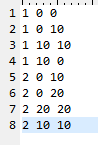
\includegraphics[width=4cm]{pictures/textak.PNG} 
\caption[Ukázka vstupního textového souboruí]{Ukázka vstupního textového souboru}
\label{fig:textak}
\end{center}
\end{figure}

%% -------<<< 4. KAPITOLA = Ukázka aplikace >>>-------\\%%
\newpage
\fancyhead[RE, RO]{\fancyplain{}{\small \sl{UKÁZKA APLIKACE}}}

\vspace*{-1cm}
\section{Ukázka aplikace}
\noindent
\large
Do této kapitolky je zahrnuto několik ukázek vytvořené aplikace. Nejprve jsou ukázany případy na datech, které nevykazují žádnou singularitu. Polygon A je vyznačen zelenou barvou, polygon B modrou barvou.

\vspace{0.2cm}
\begin{figure}[hbt!] 
\begin{center}
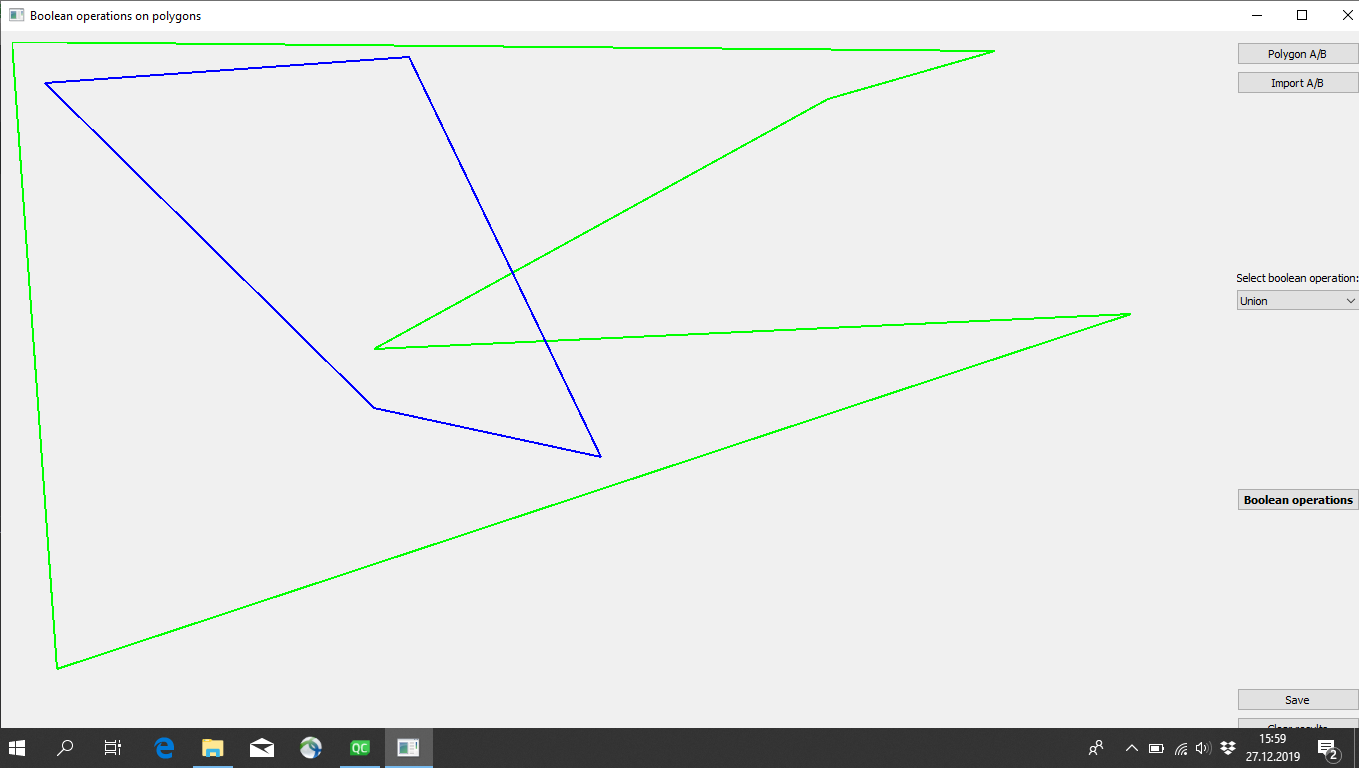
\includegraphics[width=13cm]{pictures/import_polygonu.png}
\caption[Ukázka aplikace po importu polygonů]{Ukázka aplikace po importu polygonů}
\label{fig:import_polygonu}
\end{center}
\end{figure}

\vspace{0.2cm}
\begin{figure}[hbt!] 
\begin{center}
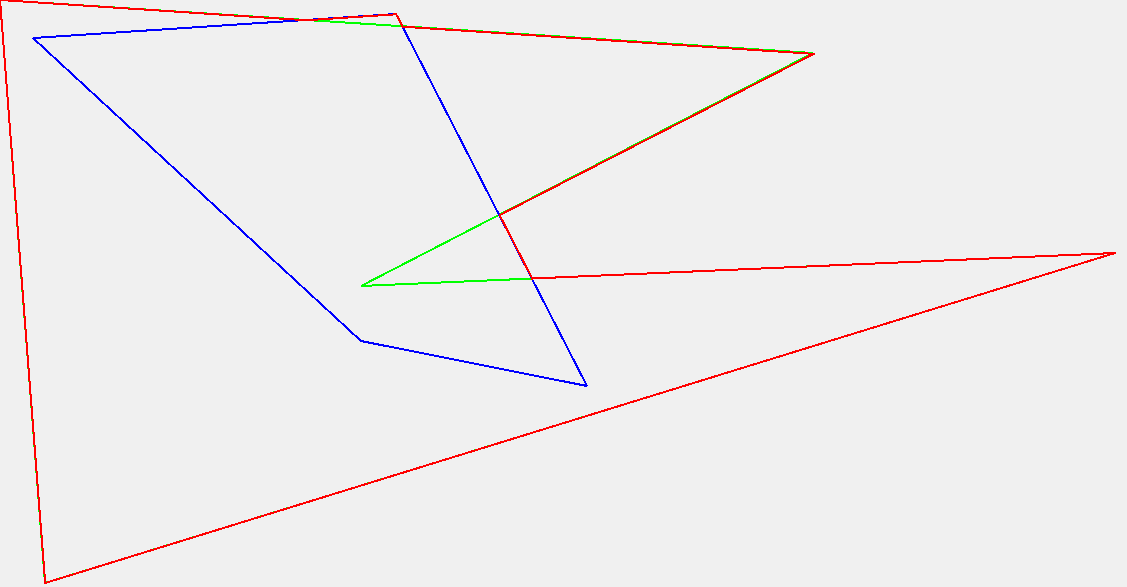
\includegraphics[width=13cm]{pictures/polygon_union.png} 
\caption[Sjednocení dvou polygonů]{Sjednocení dvou polygonů}
\label{fig:polygon_union}
\end{center}
\end{figure}

\begin{figure}[hbt!] 
\begin{center}
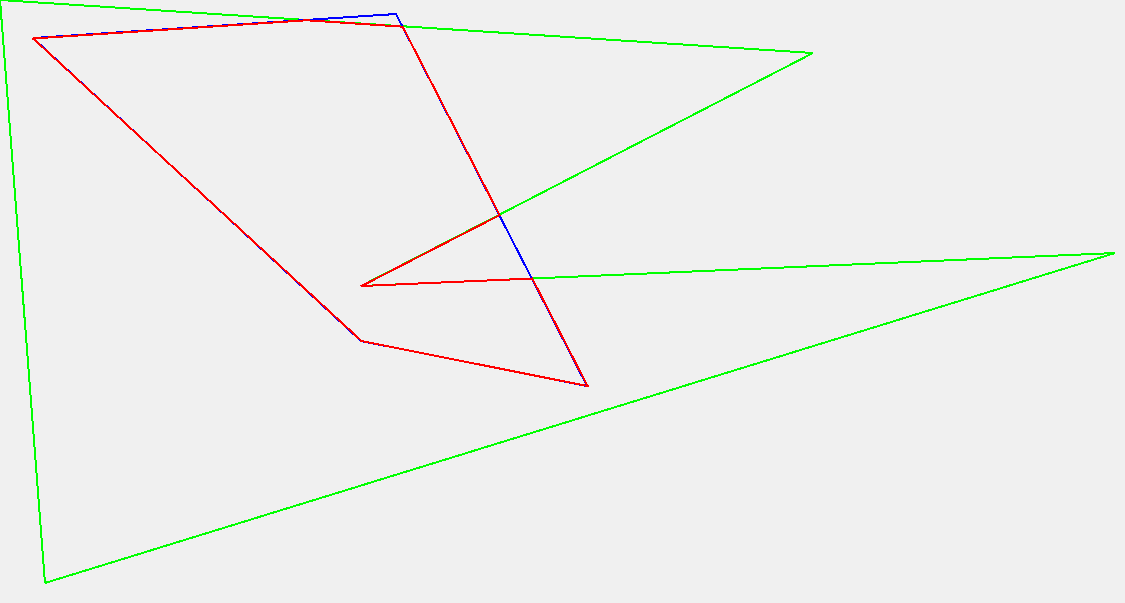
\includegraphics[width=11cm]{pictures/polygon_intersect.png} 
\caption[Průnik dvou polygonů]{Průnik dvou polygonů}
\label{fig:polygon_intersect}
\end{center}
\end{figure}

\begin{figure}[hbt!] 
\begin{center}
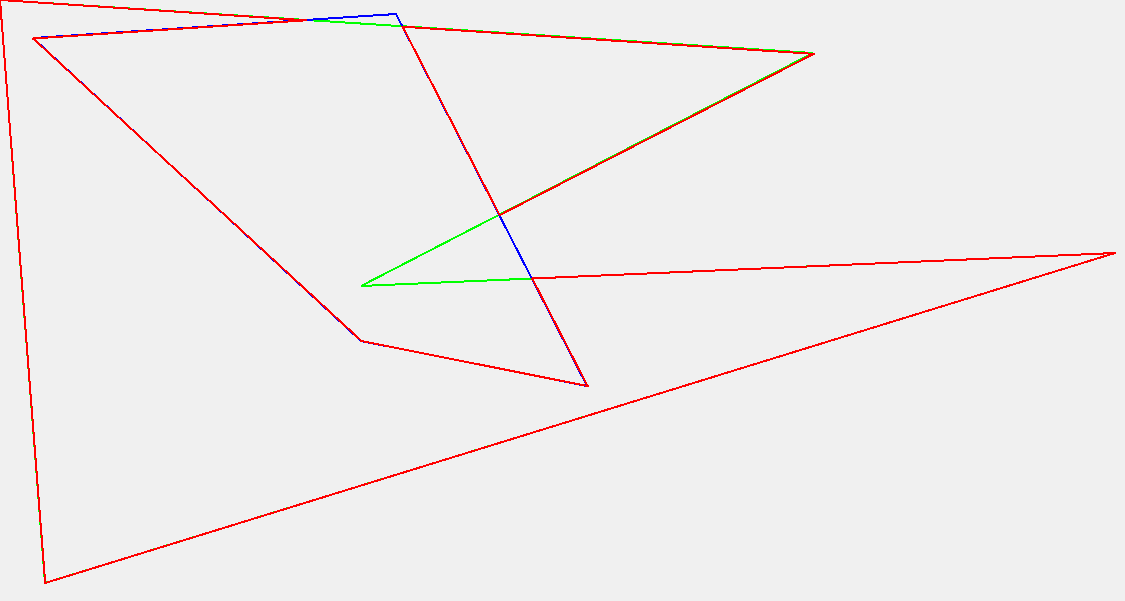
\includegraphics[width=11cm]{pictures/polygon_diffAB.png} 
\caption[Rozdíl A-B dvou polygonů A, B]{Rozdíl A-B dvou polygonů A, B}
\label{fig:polygon_diffAB}
\end{center}
\end{figure}

\begin{figure}[hbt!] 
\begin{center}
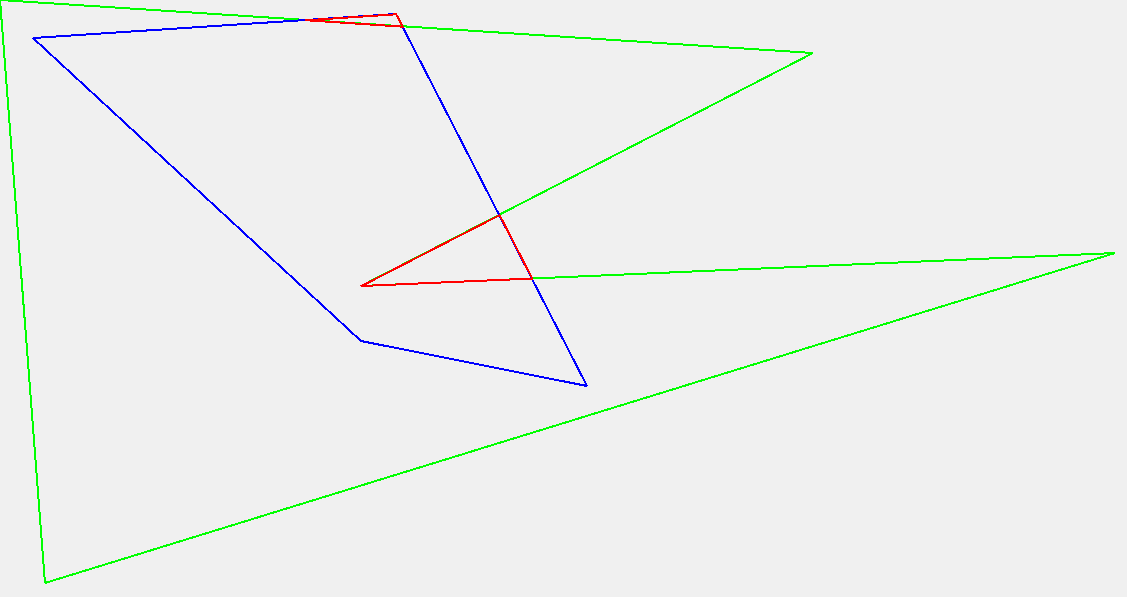
\includegraphics[width=10.5cm]{pictures/polygon_diffBA.png} 
\caption[Rozdíl B-A dvou polygonů A, B]{Rozdíl B-A dvou polygonů A, B}
\label{fig:polygon_diffBA}
\end{center}
\end{figure}

V následujících ukázkách jsou ukázany příklady singulárních situací, tak jak byly ukázány na obrázku \ref{fig:problem}. První obrázek A ukazuje situaci, kdy oba polygony mají jeden společný bod. Pokud je průsečíkem pouze 0D entita, není v aplikaci zobrazeno nic. Aplikace se soustředí pouze na společné úsečky nebo polygony. Při průniku tedy není žádná část obou polygonů zobrazena červeně, viz obrázek \ref{fig:A_intersect}.

\vspace{0.2cm}
\begin{figure}[hbt!] 
\begin{center}
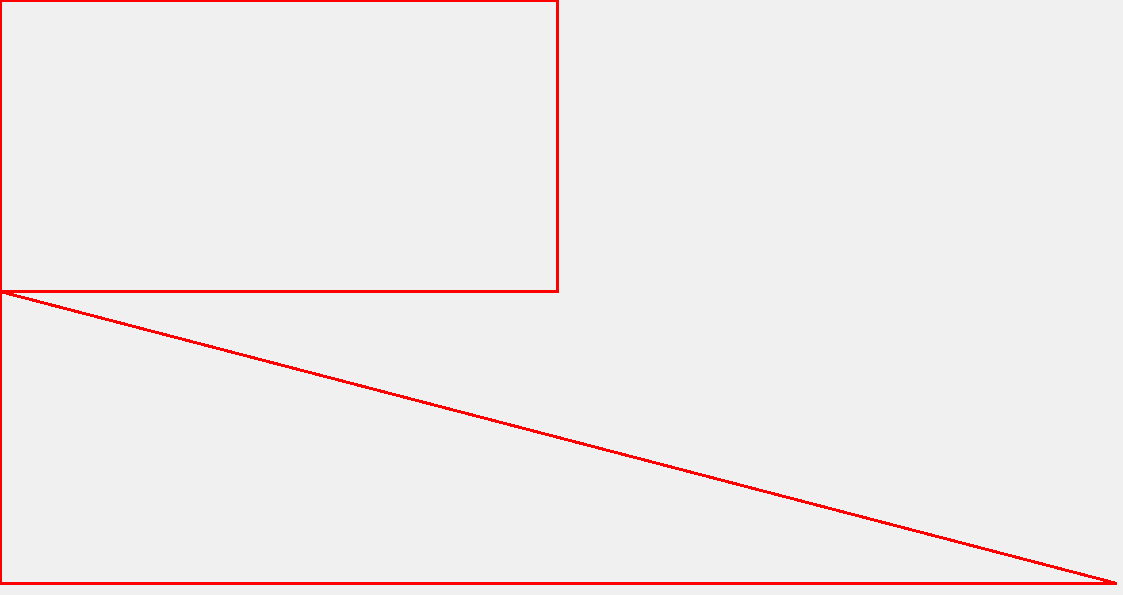
\includegraphics[width=14cm]{pictures/A_union.png} 
\caption[Situace A - společný bod - sjednocení]{Situace A - společný bod - sjednocení}
\label{fig:A_union}
\end{center}
\end{figure}

\vspace{0.2cm}
\begin{figure}[hbt!] 
\begin{center}
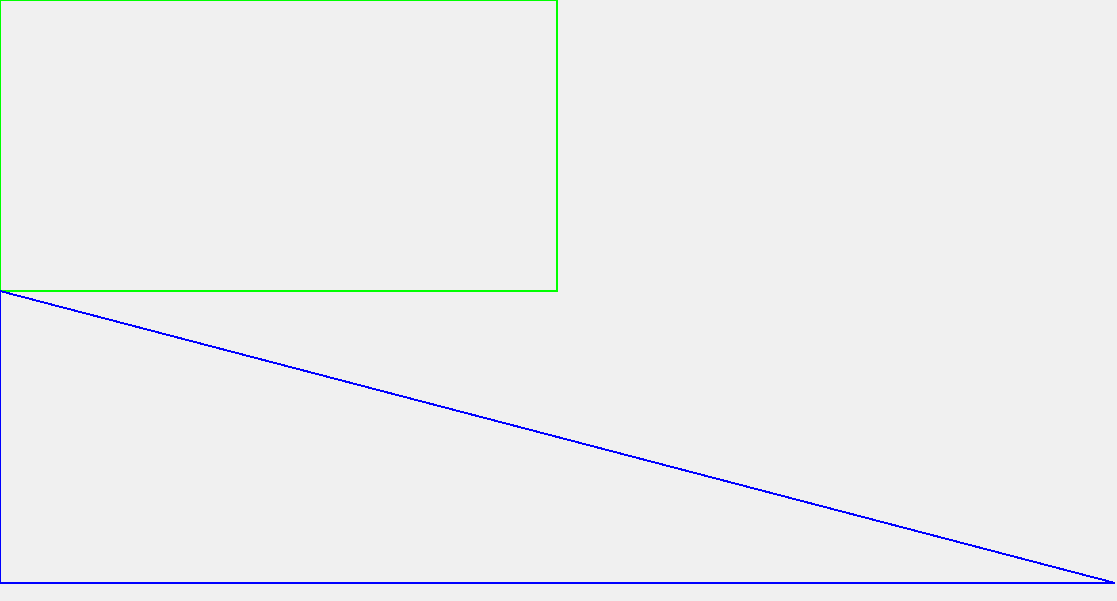
\includegraphics[width=14cm]{pictures/A_intersect.png} 
\caption[Situace A - společný bod - průnik]{Situace A - společný bod - průnik}
\label{fig:A_intersect}
\end{center}
\end{figure}

\vspace{0.2cm}
\begin{figure}[hbt!] 
\begin{center}
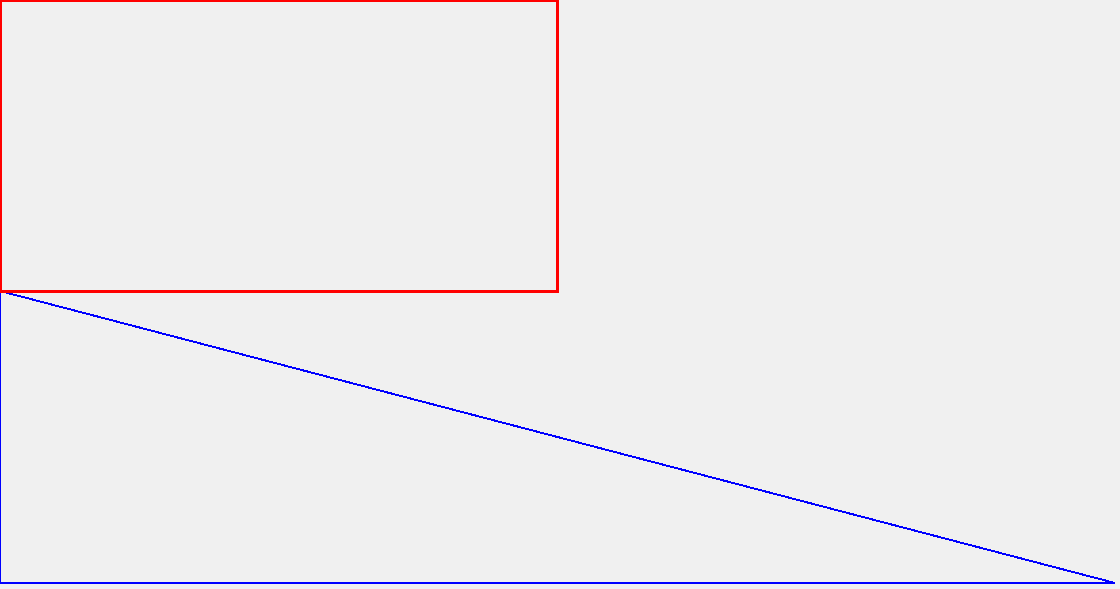
\includegraphics[width=10cm]{pictures/A_diffAB.png} 
\caption[Situace A - společný bod - rozdíl A-B]{Situace A - společný bod - rozdíl A-B}
\label{fig:A_diffAB}
\end{center}
\end{figure}

\vspace{0.2cm}
\begin{figure}[hbt!] 
\begin{center}
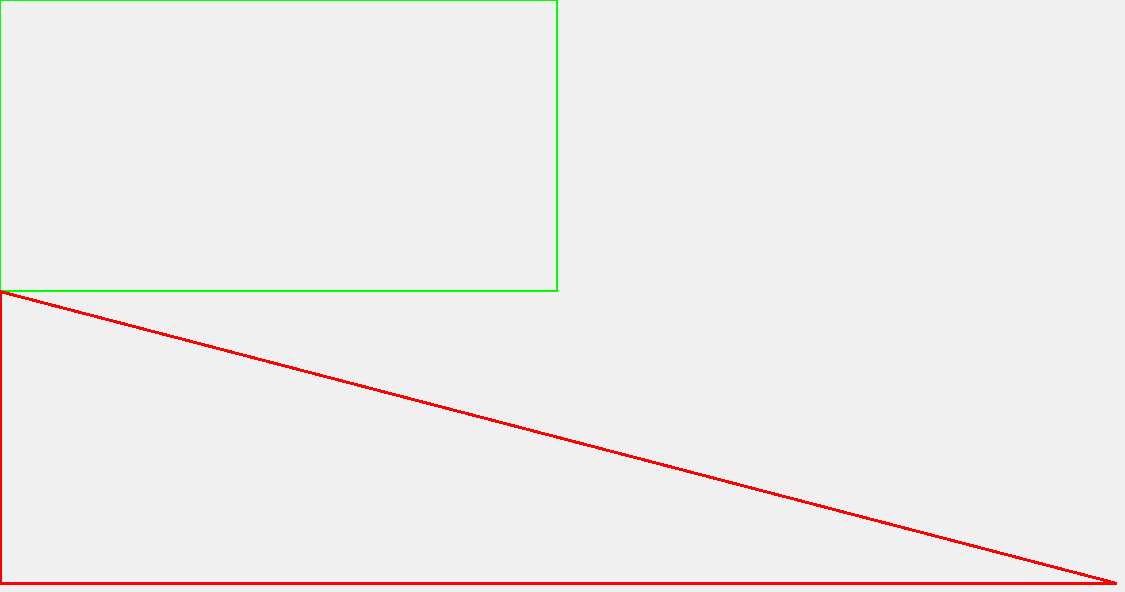
\includegraphics[width=10cm]{pictures/A_diffBA.png} 
\caption[Situace A - společný bod - rozdíl B-A]{Situace A - společný bod - rozdíl B-A}
\label{fig:A_diffBA}
\end{center}
\end{figure}

Velice podobná je situace při více společných bodech. 

\vspace{0.2cm}
\begin{figure}[hbt!] 
\begin{center}
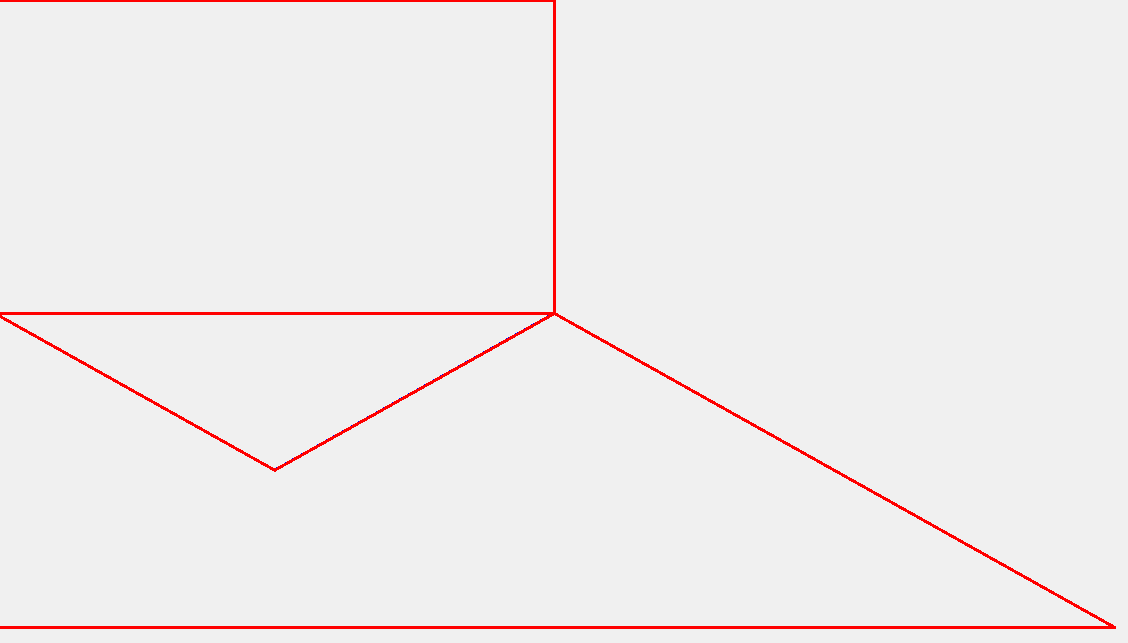
\includegraphics[width=10cm]{pictures/B_union.png} 
\caption[Situace B - více společných bodů - sjednocení]{Situace B - více společných bodů  - sjednocení}
\label{fig:B_union}
\end{center}
\end{figure}

\vspace{0.2cm}
\begin{figure}[hbt!] 
\begin{center}
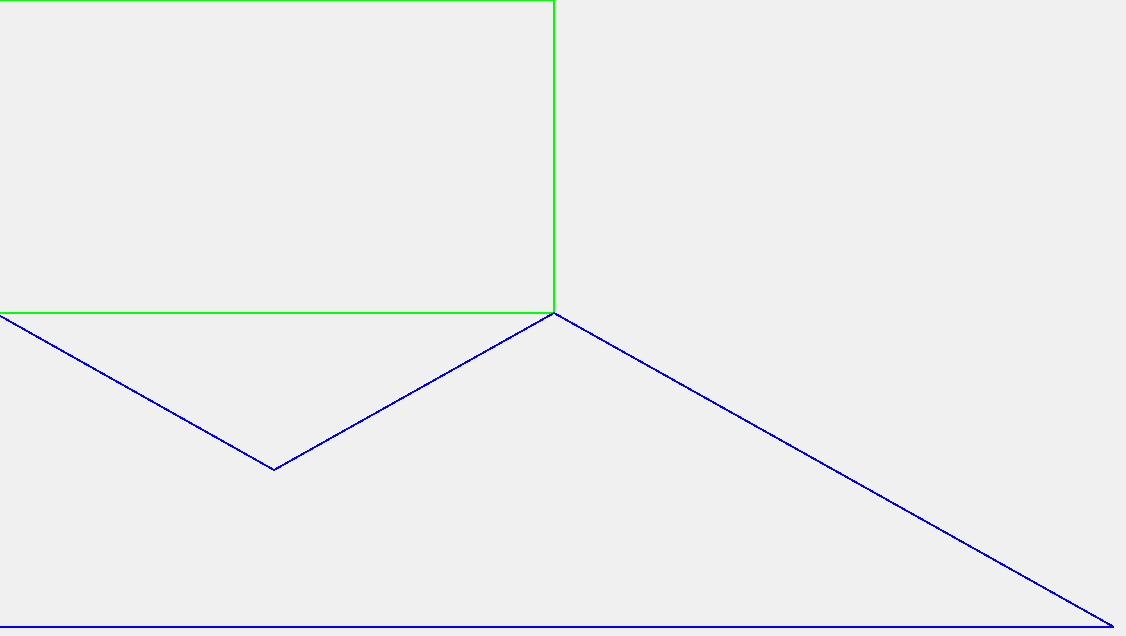
\includegraphics[width=10cm]{pictures/B_intersect.png} 
\caption[Situace B - více společných bodů  - průnik]{Situace B - více společných bodů  - průnik}
\label{fig:B_intersect}
\end{center}
\end{figure}

\vspace{0.2cm}
\begin{figure}[hbt!] 
\begin{center}
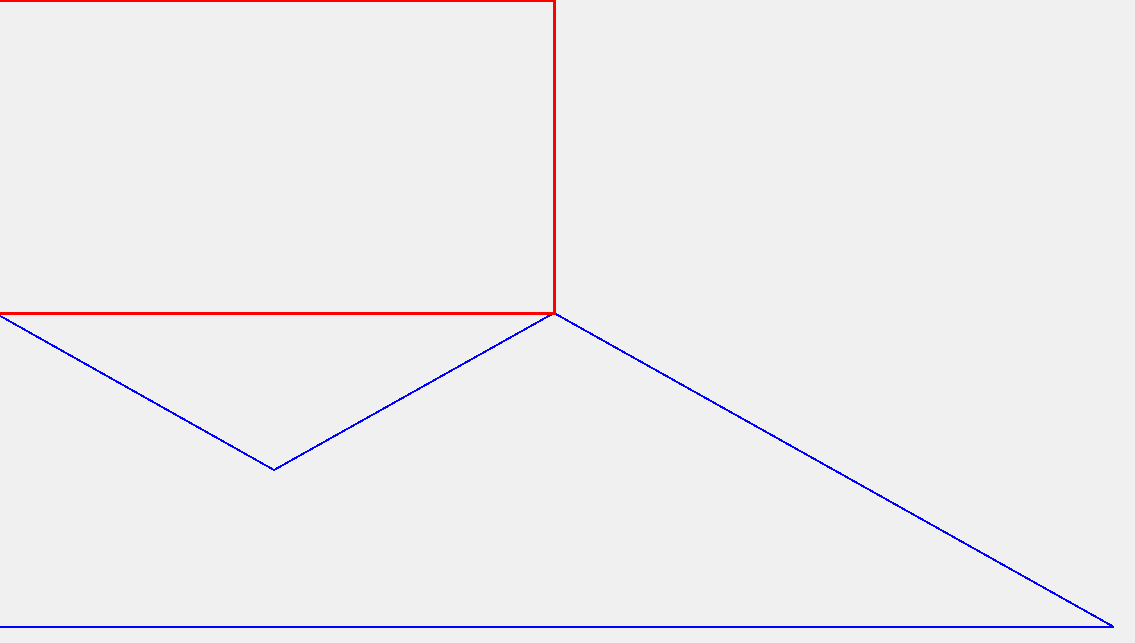
\includegraphics[width=10cm]{pictures/B_diffAB.png} 
\caption[Situace B - více společných bodů  - rozdíl A-B]{Situace B - více společných bodů  - rozdíl A-B}
\label{fig:B_diffAB}
\end{center}
\end{figure}

\vspace{0.2cm}
\begin{figure}[hbt!] 
\begin{center}
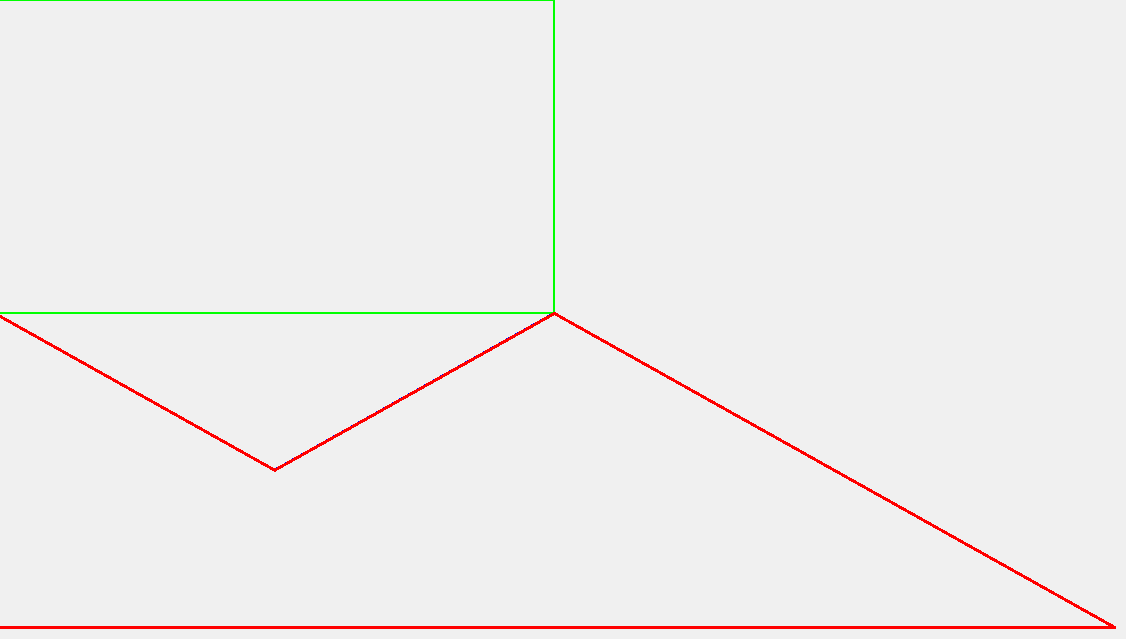
\includegraphics[width=10cm]{pictures/B_diffBA.png} 
\caption[Situace B - více společných bodů  - rozdíl B-A]{Situace B - více společných bodů  - rozdíl B-A}
\label{fig:B_diffBA}
\end{center}
\end{figure}

Polygony nemusí mít společný bod ve vrcholu, ale i v hraně. To je v tom případě, pokud se vrchol jednoho polygonu dotýká hrany druhého polygonu. V tomto případě je opět průnikem bod, který není v aplikaci vyznačen. 

\vspace{0.2cm}
\begin{figure}[hbt!] 
\begin{center}
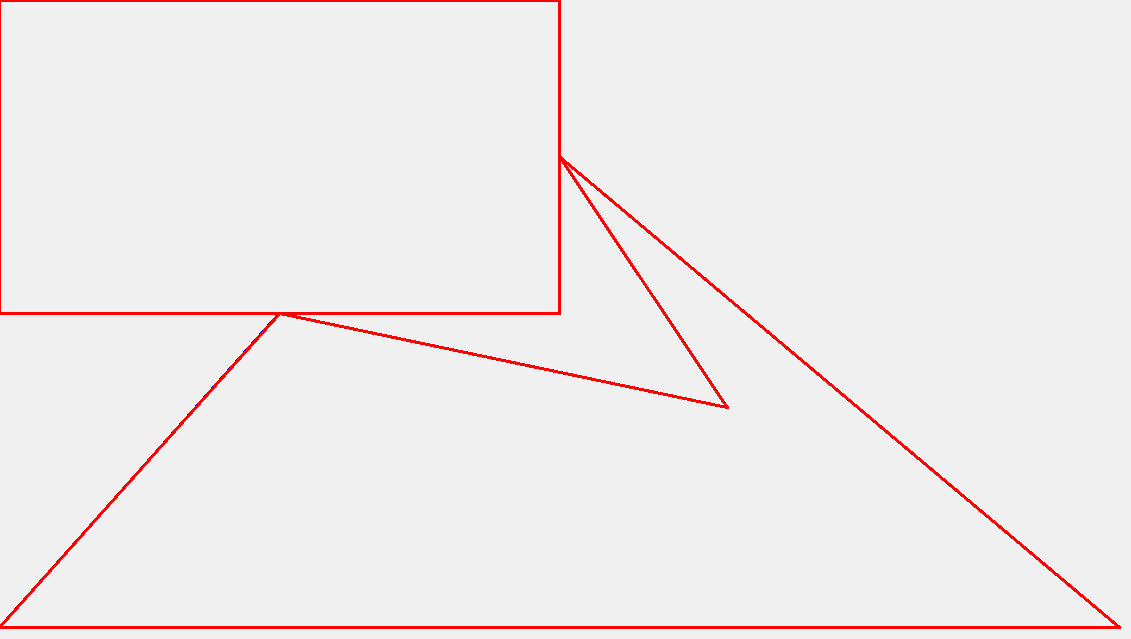
\includegraphics[width=14cm]{pictures/C_union.png} 
\caption[Situace C - body ve hraně druhého polygonu - sjednocení]{Situace C - body ve hraně druhého polygonu - sjednocení}
\label{fig:C_union}
\end{center}
\end{figure}

\vspace{0.2cm}
\begin{figure}[hbt!] 
\begin{center}
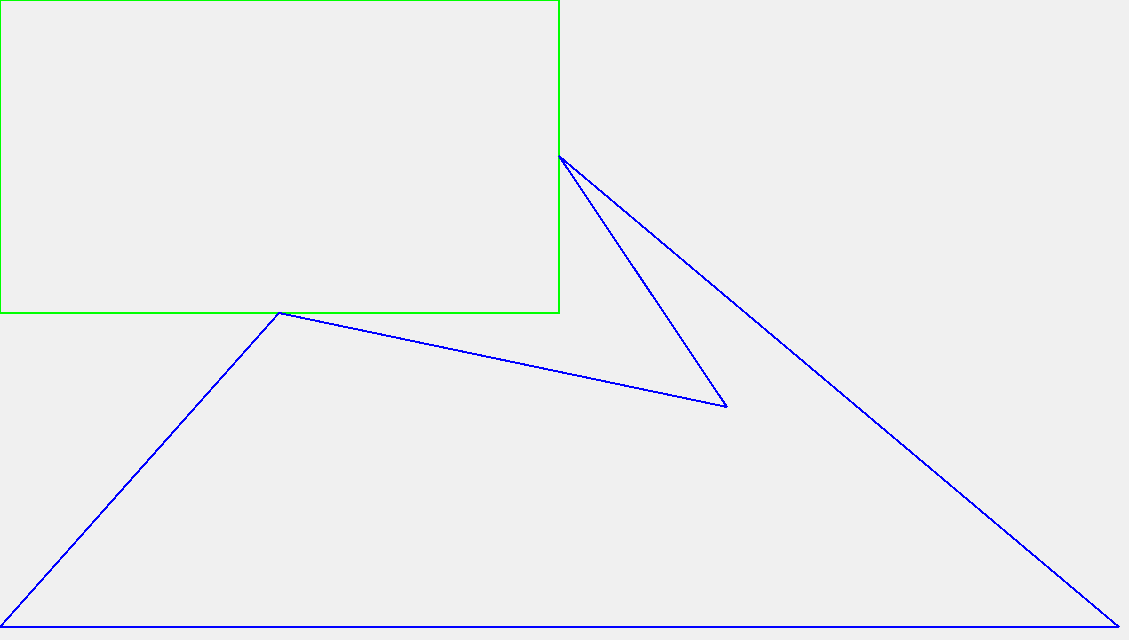
\includegraphics[width=14cm]{pictures/C_intersect.png} 
\caption[Situace C - body ve hraně druhého polygonu - průnik]{Situace C - body ve hraně druhého polygonu - průnik}
\label{fig:C_intersect}
\end{center}
\end{figure}

\vspace{0.2cm}
\begin{figure}[hbt!] 
\begin{center}
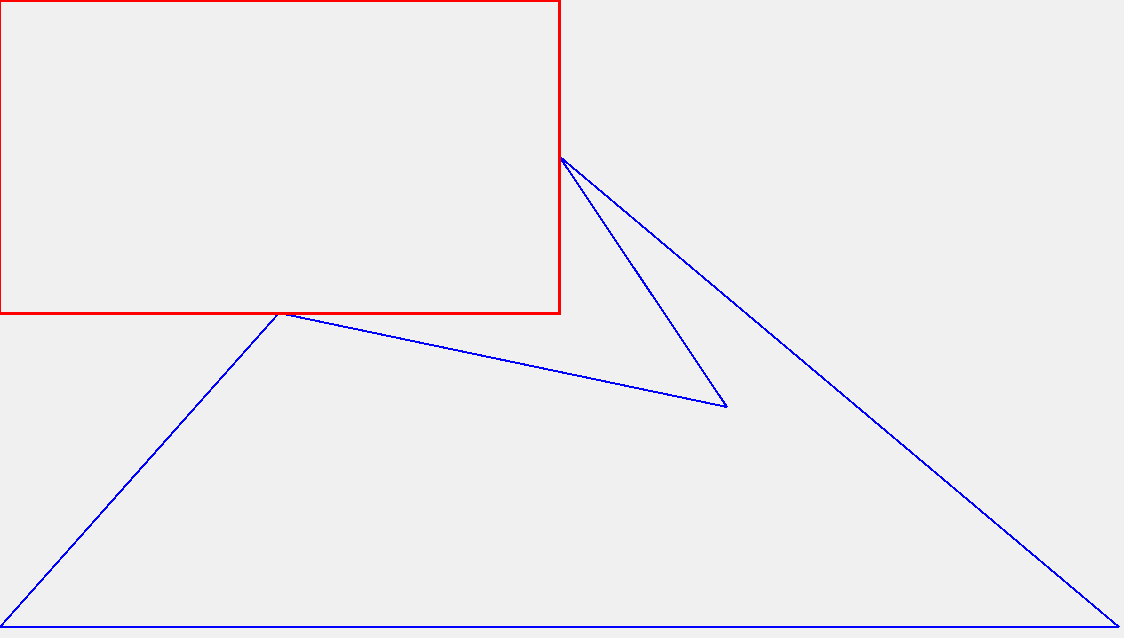
\includegraphics[width=15cm]{pictures/C_diffAB.png} 
\caption[Situace C - body ve hraně druhého polygonu - rozdíl A-B]{Situace C - body ve hraně druhého polygonu - rozdíl A-B}
\label{fig:C_diffAB}
\end{center}
\end{figure}

\vspace{0.2cm}
\begin{figure}[hbt!] 
\begin{center}
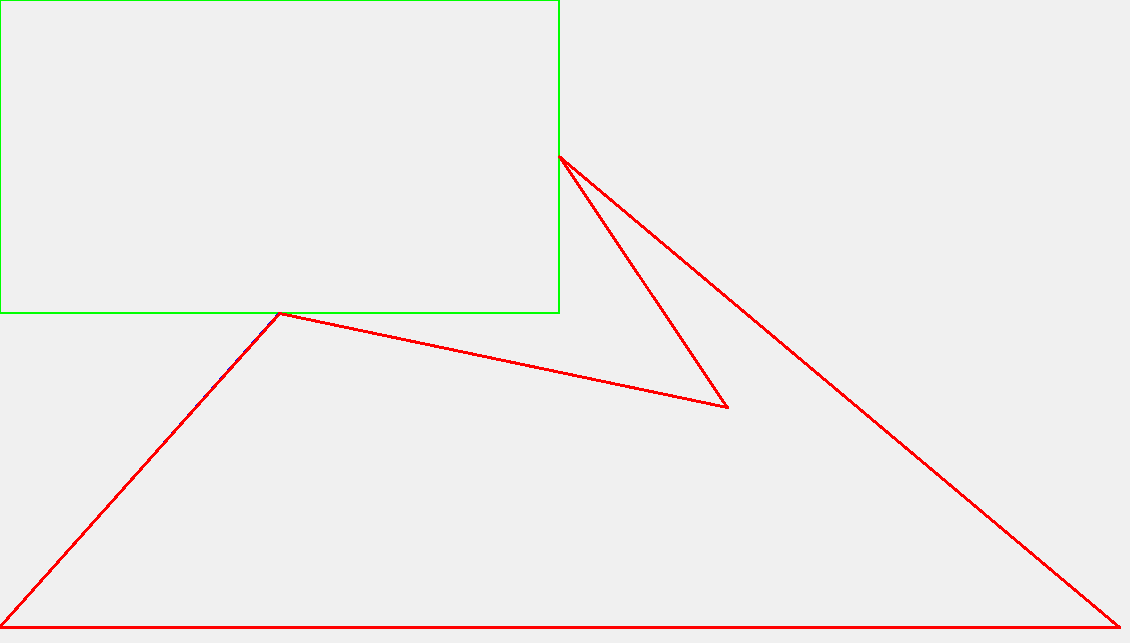
\includegraphics[width=15cm]{pictures/C_diffBA.png} 
\caption[Situace C - body ve hraně druhého polygonu - rozdíl B-A]{Situace C - body ve hraně druhého polygonu - rozdíl B-A}
\label{fig:C_diffBA}
\end{center}
\end{figure}

Dále může nastat případ, kdy se hrana jednoho polygonu přesně shoduje s hranou druhého polygonu. Průnikem takové situace je potom ona hrana. Do sjednocení obou polygonů tato hrana patří taktéž.

\vspace{0.2cm}
\begin{figure}[hbt!] 
\begin{center}
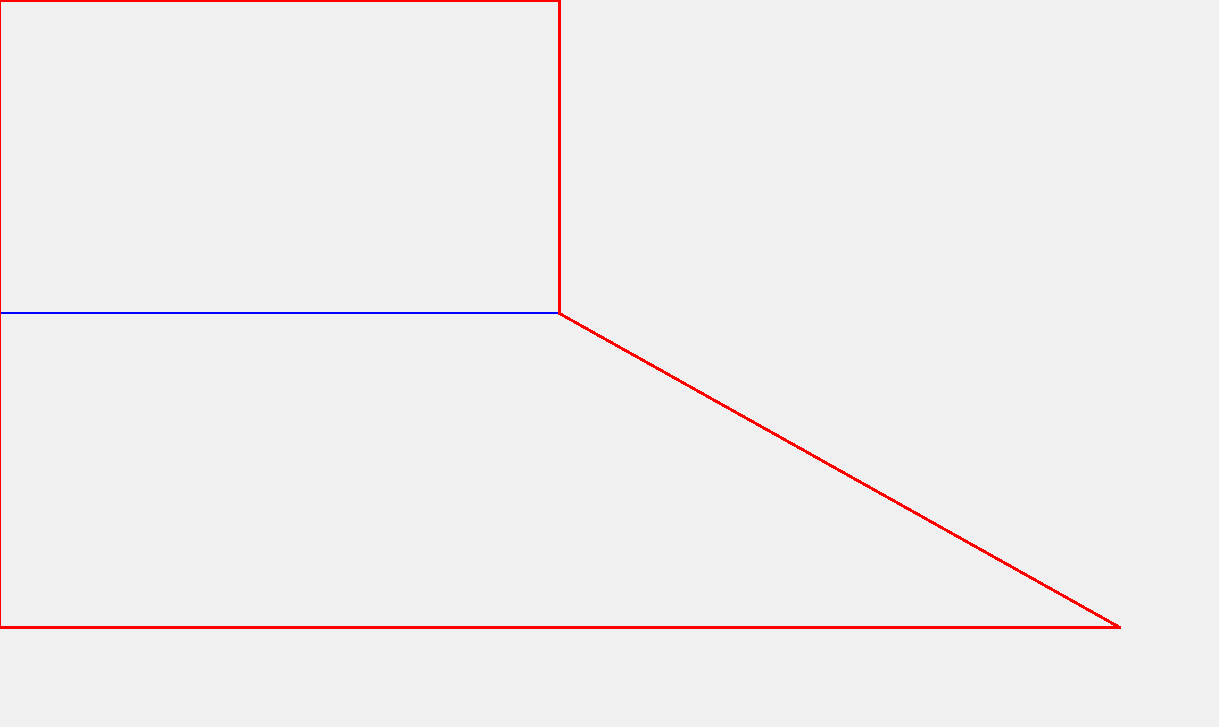
\includegraphics[width=10cm]{pictures/D_union_v2.png} 
\caption[Situace D - hrana obou polygonů se shoduje - sjednocení]{Situace D - hrana obou polygonů se shoduje - sjednocení}
\label{fig:D_union}
\end{center}
\end{figure}

\vspace{0.2cm}
\begin{figure}[hbt!] 
\begin{center}
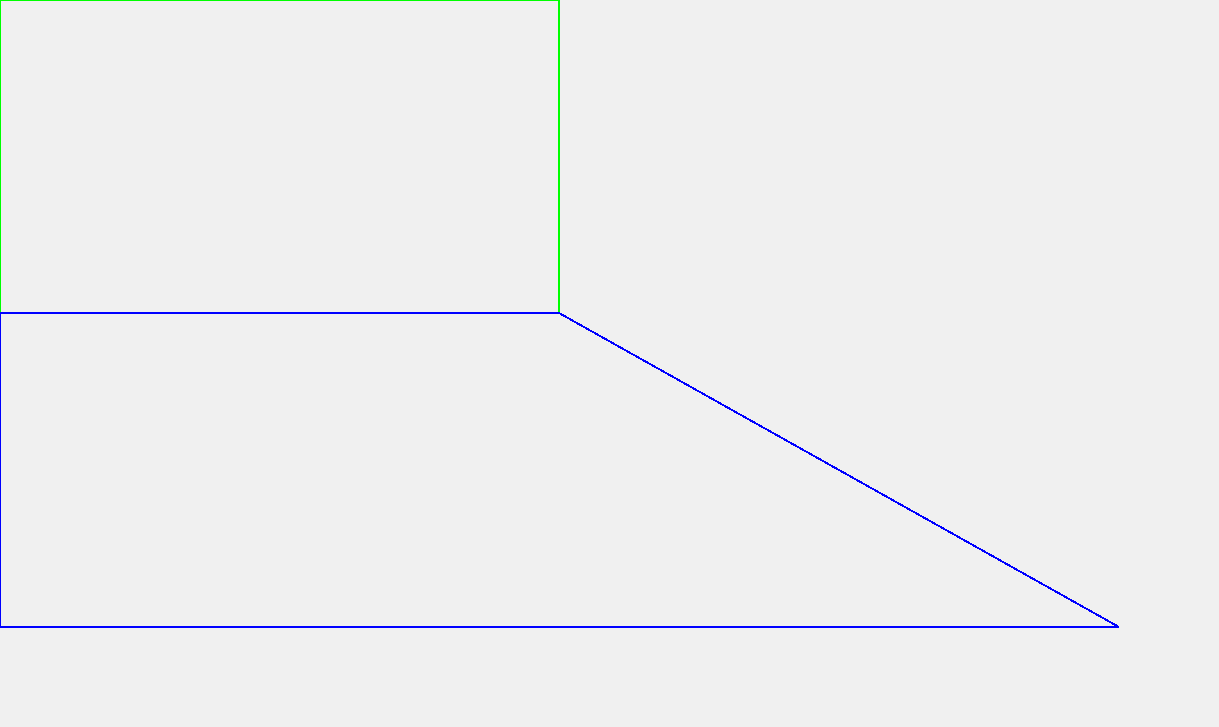
\includegraphics[width=10cm]{pictures/D_intersect_v2.png} 
\caption[Situace D - hrana obou polygonů se shoduje - průnik]{Situace D - hrana obou polygonů se shoduje - průnik}
\label{fig:D_intersect}
\end{center}
\end{figure}

\vspace{0.2cm}
\begin{figure}[hbt!] 
\begin{center}
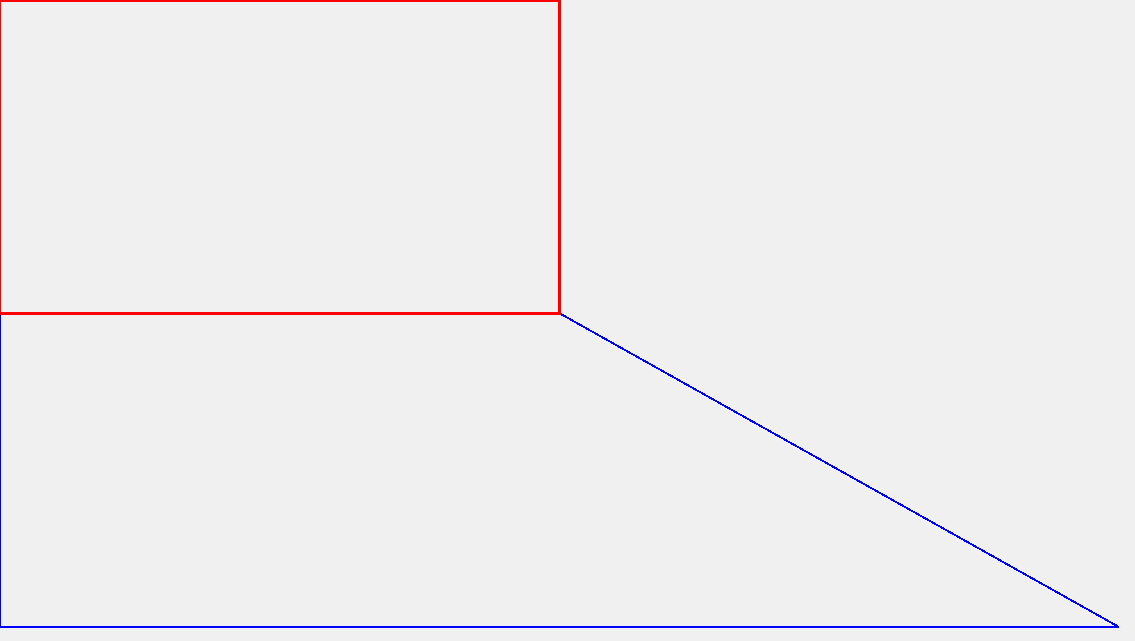
\includegraphics[width=10cm]{pictures/D_diffAB.png} 
\caption[Situace D - hrana obou polygonů se shoduje - rozdíl A-B]{Situace D - hrana obou polygonů se shoduje - rozdíl A-B}
\label{fig:D_diffAB}
\end{center}
\end{figure}

\vspace{0.2cm}
\begin{figure}[hbt!] 
\begin{center}
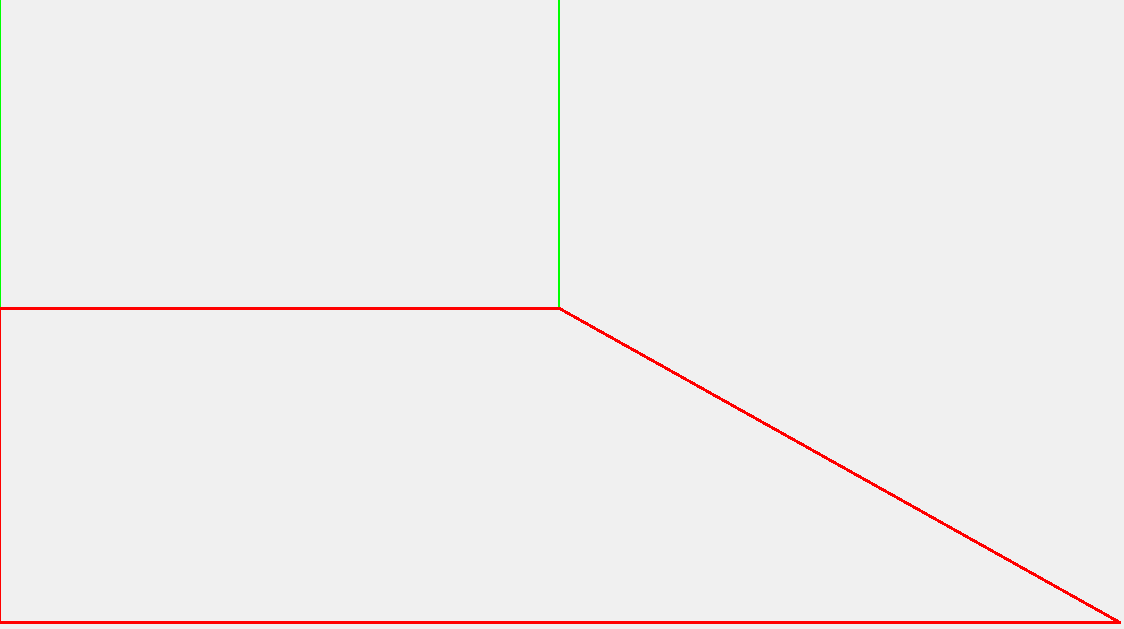
\includegraphics[width=10cm]{pictures/D_diffBA.png} 
\caption[Situace D - hrana obou polygonů se shoduje - rozdíl B-A]{Situace D - hrana obou polygonů se shoduje - rozdíl B-A}
\label{fig:D_diffBA}
\end{center}
\end{figure}

Dalšími singulárními případy je společná část hrany [E] nebo hrana ležící v hraně druhého polygonu [F]. Oba tyto případy jsou velmi podobné případu D.

\vspace{0.2cm}
\begin{figure}[hbt!] 
\begin{center}
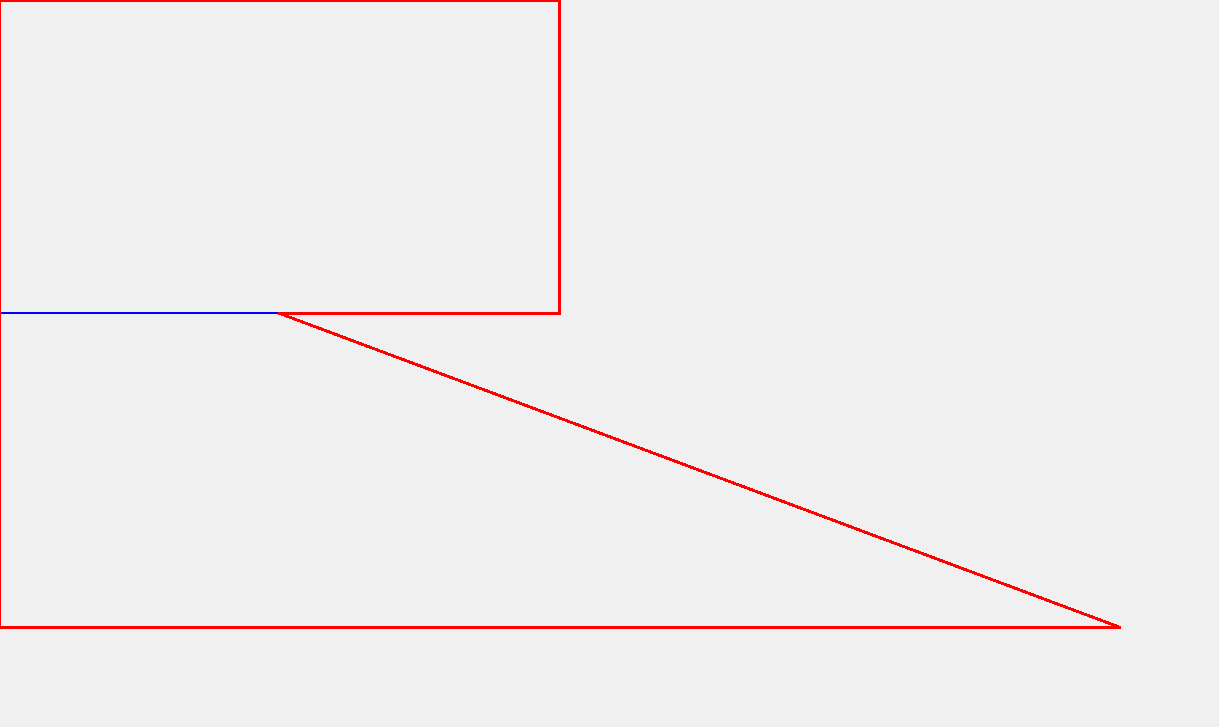
\includegraphics[width=10cm]{pictures/E_union_v2.png} 
\caption[Situace E - společná část hrany - sjednocení]{Situace E - společná část hrany - sjednocení}
\label{fig:E_union}
\end{center}
\end{figure}

\vspace{0.2cm}
\begin{figure}[hbt!] 
\begin{center}
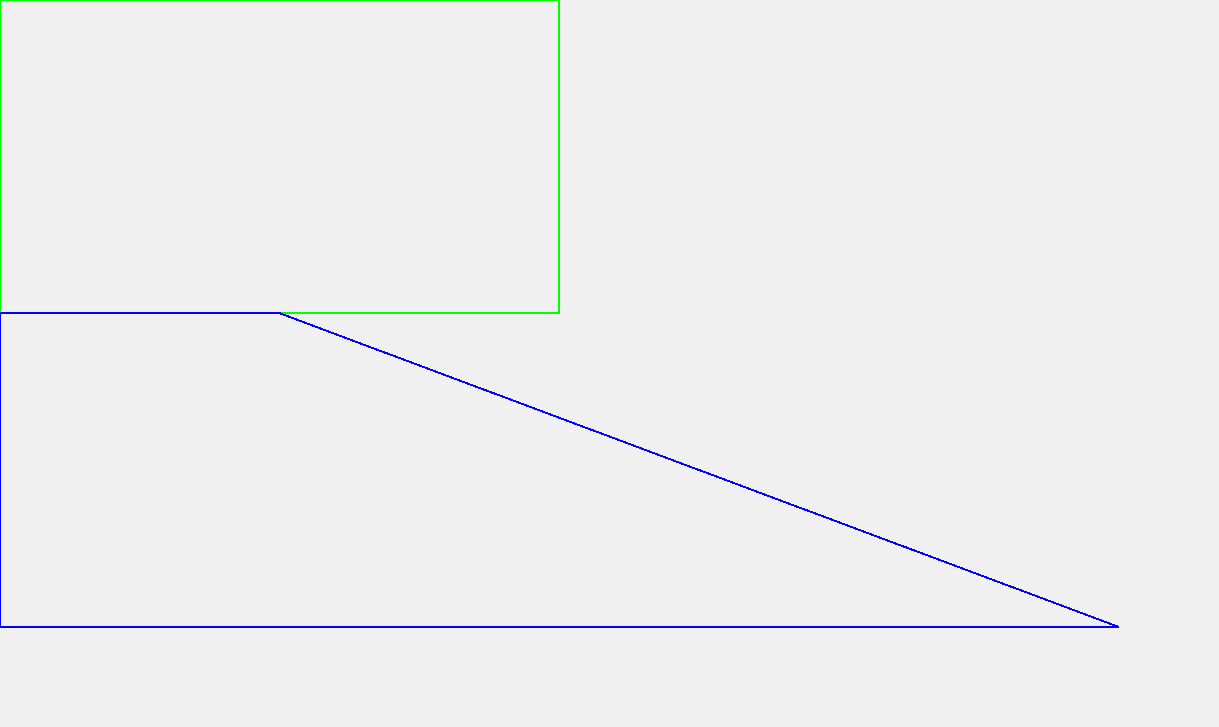
\includegraphics[width=9cm]{pictures/E_intersect_v2.png} 
\caption[Situace E - společná část hrany - průnik]{Situace E - společná část hrany - průnik}
\label{fig:E_intersect}
\end{center}
\end{figure}

\vspace{0.2cm}
\begin{figure}[hbt!] 
\begin{center}
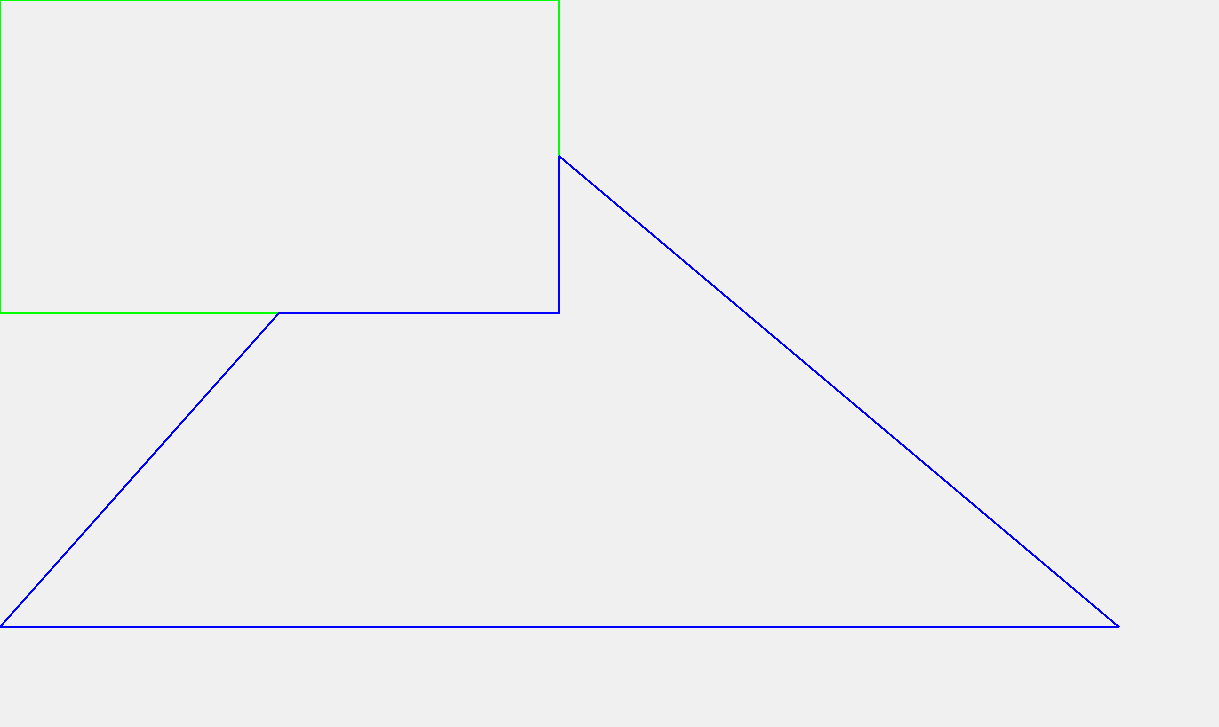
\includegraphics[width=10cm]{pictures/E_more_intersect_v2.png} 
\caption[Situace E - společná část více hran - průnik]{Situace E - společná část více hran - průnik}
\label{fig:E_more_intersect}
\end{center}
\end{figure}

\vspace{0.2cm}
\begin{figure}[hbt!] 
\begin{center}
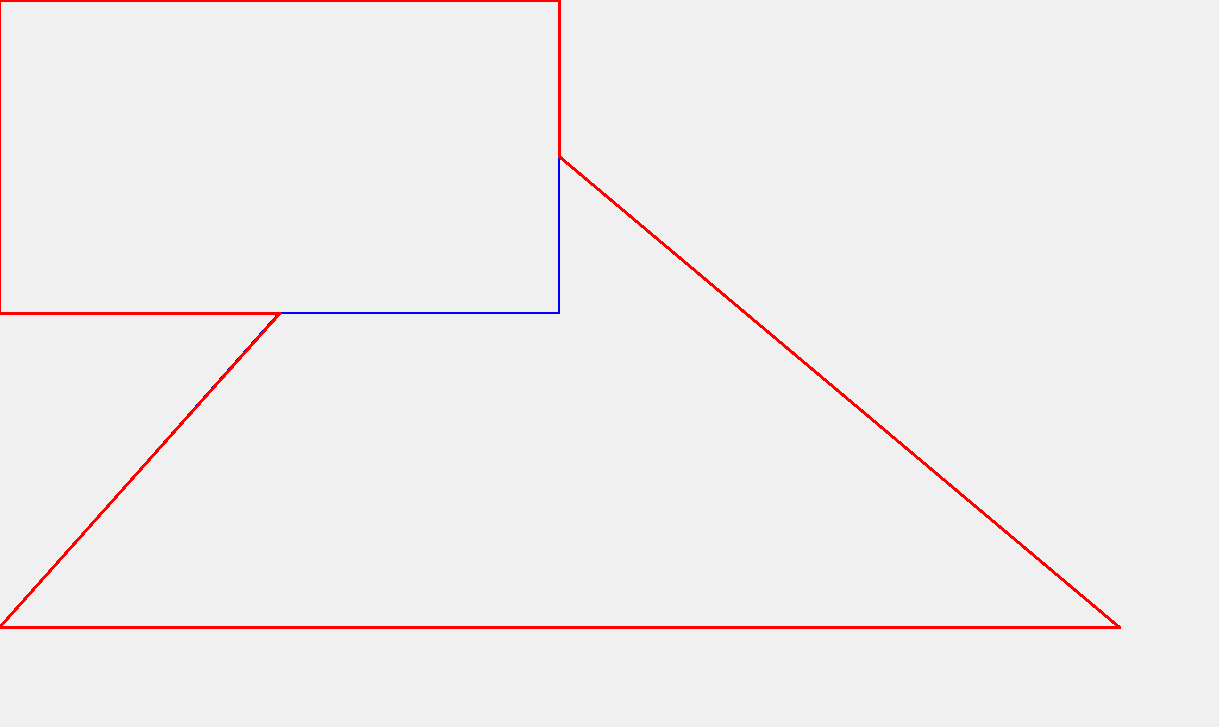
\includegraphics[width=10cm]{pictures/E_more_union_v2.png} 
\caption[Situace E - společná část více hran - sjednocení]{Situace E - společná část více hran - sjednocení}
\label{fig:E_more_union}
\end{center}
\end{figure}

\vspace{0.2cm}
\begin{figure}[hbt!] 
\begin{center}
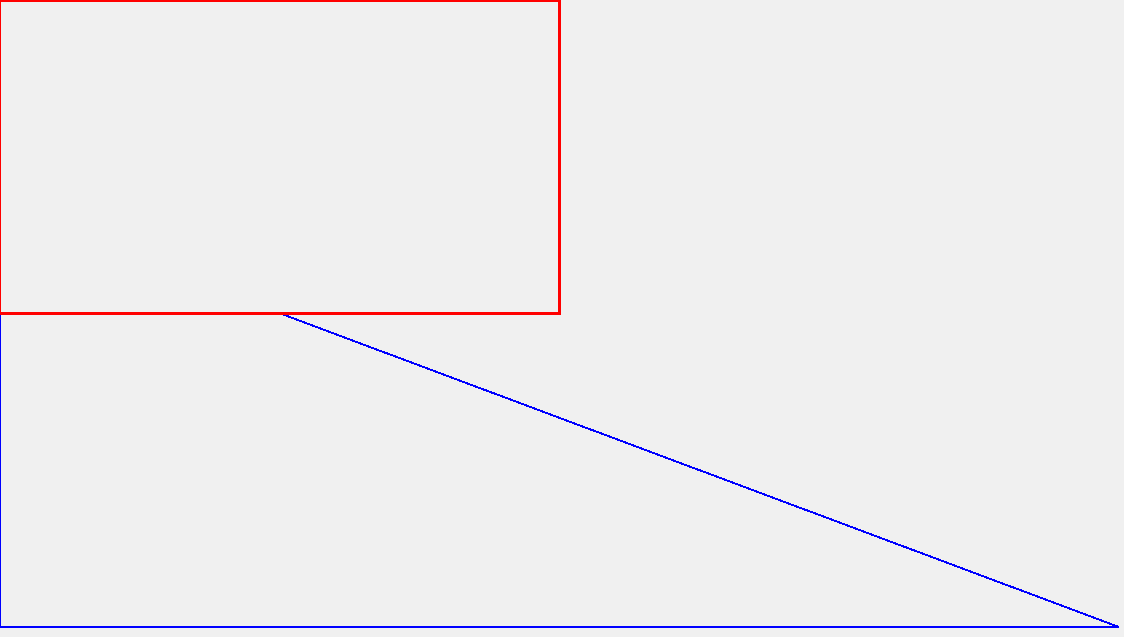
\includegraphics[width=10cm]{pictures/E_diffAB.png} 
\caption[Situace E - společná část hrany - rozdíl A-B]{Situace E - společná část hrany - rozdíl A-B}
\label{fig:E_diffAB}
\end{center}
\end{figure}

\vspace{0.2cm}
\begin{figure}[hbt!] 
\begin{center}
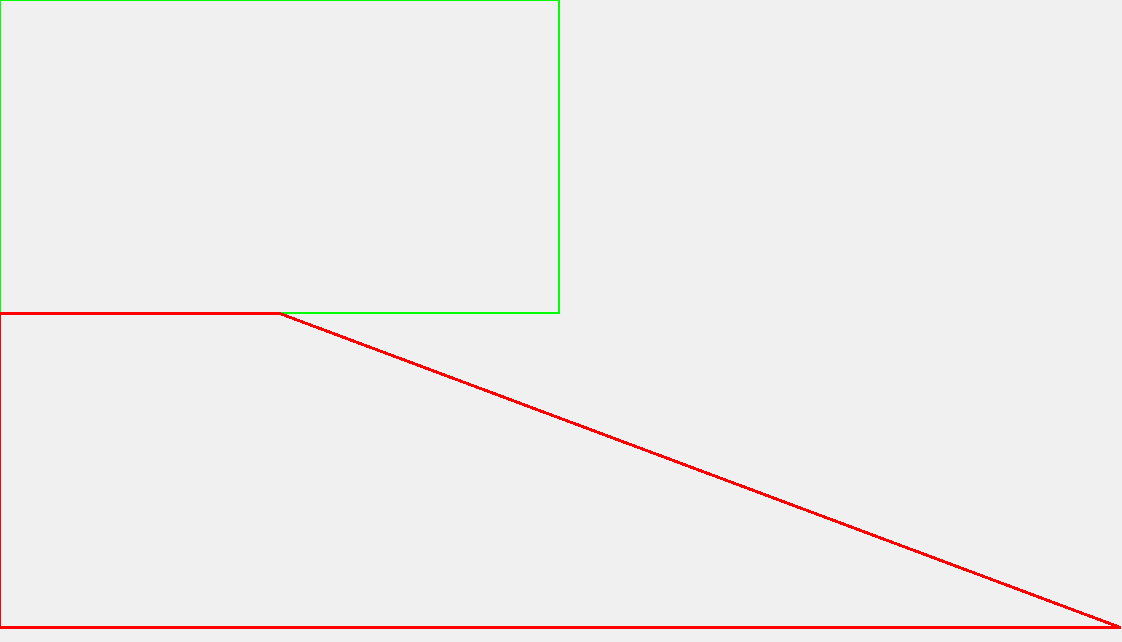
\includegraphics[width=10cm]{pictures/E_diffBA.png} 
\caption[Situace E - společná část hrany - rozdíl B-A]{Situace E - společná část hrany - rozdíl B-A}
\label{fig:E_diffBA}
\end{center}
\end{figure}

\vspace{0.2cm}
\begin{figure}[hbt!] 
\begin{center}
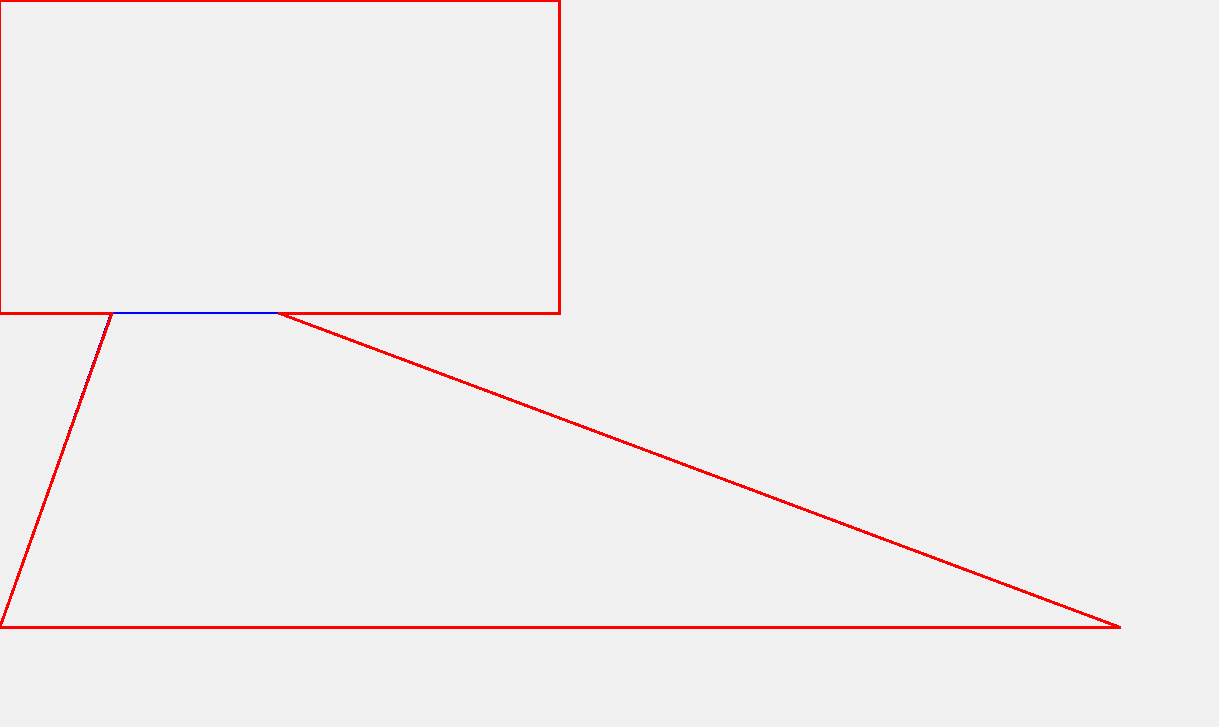
\includegraphics[width=10cm]{pictures/F_union_v2.png} 
\caption[Situace F - hrana ležící v hraně druhého polygonu - sjednocení]{Situace F - hrana ležící v hraně druhého polygonu - sjednocení}
\label{fig:F_union}
\end{center}
\end{figure}

\vspace{0.2cm}
\begin{figure}[hbt!] 
\begin{center}
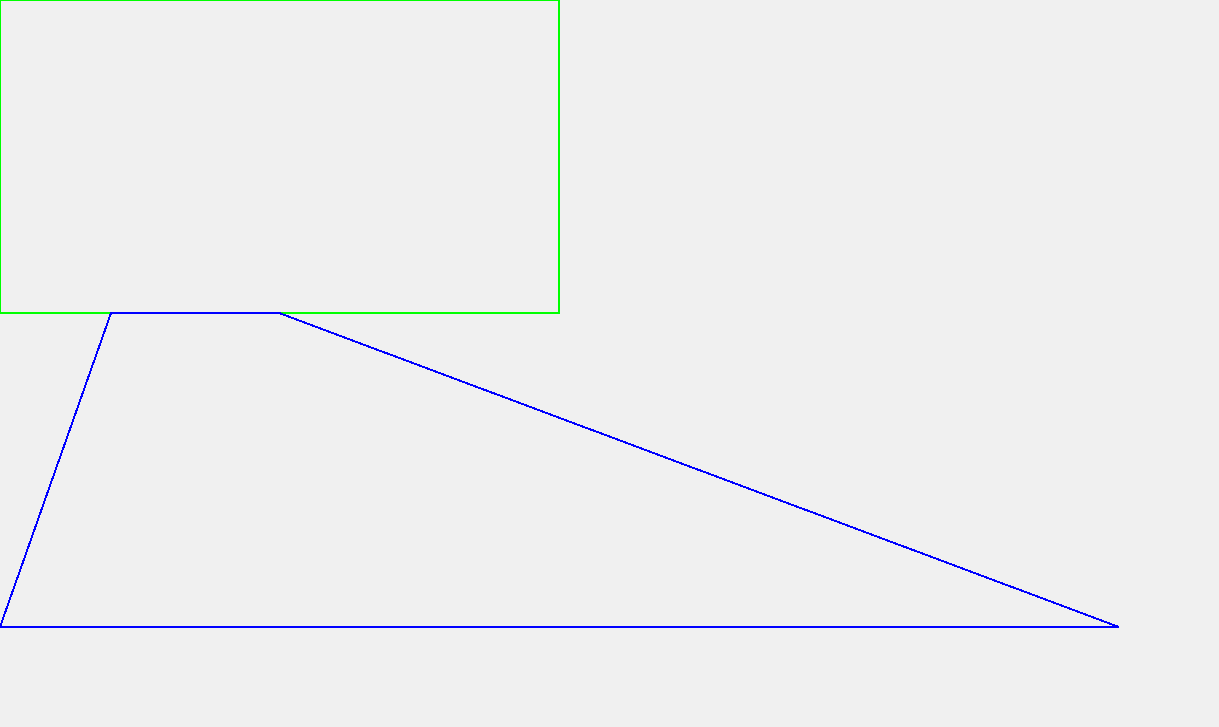
\includegraphics[width=9cm]{pictures/F_intersect_v2.png} 
\caption[Situace F - hrana ležící v hraně druhého polygonu - průnik]{Situace F - hrana ležící v hraně druhého polygonu - průnik}
\label{fig:F_intersect}
\end{center}
\end{figure}

%% -------<<< 5. KAPITOLA = Technická dokumentace >>>-------\\%%

\newpage
\fancyhead[RE, RO]{\fancyplain{}{\small \sl{TECHNICKÁ DOKUMENTACE}}}

\vspace*{-1cm}
\section{Technická dokumentace}
\subsection{Třídy}
V aplikaci se nachází celkem pět tříd QPointFB, Types, Algorithms, Draw a Widget. Dále se zde nachází hlavičkový soubor Types s definovanými výčtovými typy.

\subsubsection{Hlavičkový soubor Types}
V tomto hlavičkovém souboru je definováno několik výčtových typů. \\

\noindent Prvním je typ definující polohu bodu vůči přímce. Je používán ve funkci \textit{getPointLinePosition}, která je používána ve funkci \textit{positionPointPolygonWinding}.\\
\noindent\textbf{ typedef enum \{LeftHp = 0, RightHp = 1, Colinear = 2\} TPointLinePosition}\\

\noindent Druhým je typ definující polohu bodu vůči polygonu. Tento typ je návratovým typem funkce \textit{positionPointPolygonWinding}. Je rozhodujícím pro výběr hran.\\
\noindent\textbf{ typedef enum \{Inner, Outer, On\} TPointPolygonPosition}\\

\noindent Definuje typ množinové operace. Podle toho, která je zvolena, dojde ve funkci  \textit{booleanOperation} k výběru příslušných hran, které budou poté červeně zobrazeny jakožto výsledek množinové operace.\\
\noindent\textbf{ typedef enum \{Union, Intersect, DifferenceAB, DifferenceBA\} TBolleanOperation}\\

\noindent Čtvrtým je typ definující polohu bodu vůči přímce. Je použit ve funkci \textit{get2LinesPosition}, která je použita ve funkci \textit{computePolygonIntersection}. Tento tyo je tedy důležitý při výpočtu průsečíků obou polygonů.\\
\noindent\textbf{ typedef enum \{Parallel, Identical, NonIntersected, Intersected\} T2LinePosition}

\subsubsection{QPointFB}
Tato třída dědí od třídy PointF. Konstruktor se skládá ze souřadnic x,y, které jsou odvozeny od rodičovské třídy QPointF. Navíc jsou v konstruktoru inicializovány hodnoty $\alpha$ a $\beta$ a pozice bodu vůči polygonu.
\noindent Konstruktor má tvar:\\
\noindent\textbf{QPointFB(double x, double y):QPointF(x,y), alpha(0), beta(0), position(On)\{\}}\\

\noindent Ve třídě je dále definováno několik setterů a getterů:\\
\noindent\textbf{void setAlpha (double alpha\_)}\\
\noindent\textbf{void setBeta (double beta\_)}\\
\noindent\textbf{void setPosition (TPointPolygonPosition position\_)}\\
\noindent\textbf{double getAlpha()}\\
\noindent\textbf{double getBeta()}\\
\noindent\textbf{TPointPolygonPosition getPosition ()}

\newpage
\vspace*{-1cm}
\subsubsection{Algorithms}
Třída Algorithms obsahuje konstruktor a metody, které jsou určeny pro výpočet algoritmů používaných v digitálním GIS. Datové typy u bodu a polygonu byly zvoleny s plovoucí desetinnou čárkou (floating point).\\

\noindent\textbf{TPointLinePosition getPointLinePosition(QPointFB \&q, QPointFB \&p1, QPointFB \&p2)}\\
Tato funkce má za úkol určit polohu bodu \textit{q} vůči přímce zadané dvěma body \textit{p1} a \textit{p2}.  Nejprve se z vektorů vypočítá determinant. Pokud je determinant větší než tato tolerance, bod se nechází v levé polorovině a funkce vrací výčtový typ \textit{LeftHp}. Pokud je menší, bod se nachází v pravé polorovině a funkce vrací výčtový typ \textit{RightHp}.  Pokud nenastane ani jeden z výše uvedených případů, výstupem je \textit{Colinear}.\\

\noindent\textbf{double length2Points(QPointFB p, QPointFB q)}\\
Vrací vzdálenost dvou bodů vypočtenou z Pythagorovy věty.\\

\noindent\textbf{double getAngle2Vectors(QPointFB \&p1, QPointFB \&p2, \\ QPointFB \&p3, \&QPointFB p4)}\\
V této funkci je pomocí norem a skalárního součinu počítán úhel mezi dvěma hranami zadanými čtyřmi body typu QPointF. Úhel je vypočten jako arcus cosinus poměru skalárního součinu a součinu obou velikostí. Defaultně se v prostředí počítá v radiánech, což bylo ponecháno.\\

\noindent\textbf{TPointPolygonPosition positionPointPolygonWinding(QPointF \&q, QPolygonF \&pol)}\\
Tato funkce určí polohu bodu vůči polygonu metodou Winding Number Algorithm. Vstupem je určovaný bod \textit{q} a polygon \textit{P}, vůči kterému je poloha určována. Hned na počátku je také zvolena tolerance (minimální hodnota) \textit{eps = 1e-6}. V případě, že výstupem je výčtový typ \textit{Outer}, bod leží mimo polygon, v případě že \textit{Inner}, bod leží uvnitř polygonu. Pokud nenastane žádná z těchto uvedených možností, výstupem je hodnota \textit{On}. \\

\noindent\textbf{T2LinePosition get2LinesPosition(QPointFB \&p1, QPointFB \&p2, \\ QPointFB \&p3, QPointFB \&p4, QPointFB \&pi)}\\
Určí pozici dvou přímek vůči sobě. Pokud najde průsečík, uloží jej do proměnné \textit{pi} typu reference. Nejprve se z vektorů vypočítají dílčí determinanty. Pokud jsou všechny téměř nula, funkce vrátí výčtový typ \textit{Identical}. Pokud je první a druhý dílčí determinant téměř roven nule, funkce vrátí  výčtový typ \textit{Parallel}. Pokud nedojde k těmto případům, jsou vypočteny parametry alfa a beta. Pokud je alfa i beta mezi 0 a 1 včetně, je nalezen průsečík a vrácen text \textit{Intersected}. Pokud nenastane žádná z těchto variant, úsečky nemají žádný společný bod a funkce vrátí \textit{NonIntersected}.\\

\noindent\textbf{void processIntersection(QPointFB \&pi, double \&t, std::vector$<QPointFB>$ \&polygon, int \&i)}\\
Tato funkce je volána ve funkci \textit{computePolygonIntersection} a zpracovává nalezený průsečík, který má určité parametry alfa a beta a také svůj index. Podle toho se určí, na jaké místo v polygonu má být vložen.\\

\noindent\textbf{std::vector$<Edge>$ booleanOperations(std::vector$<QPointFB>$ \&polygonA,  std::vector$<QPointFB>$ \&polygonB, TBooleanOperation operation)}\\
Vrátí výsledné hrany podle požadované operace. Nejprve vrátí průsečíky obou polygonů a vloží je na své místo do polygonů (funkce \textit{computePolygonIntersection}). Poté vypočte pozici polygonu A vůči polygonu B a naopak. Pokud je vybrána operace UNION, jsou vybrány vnější hrany k polygonu A (OUTER) a vnější hrany z polygonu B pomocí funkce \textit{selectEdges}. Pokud je vybrána operace INTERSECT, jsou vybrány vnitřní hrany k polygonu A (INNER) a vnitřní hrany z polygonu B. Pokud je vybrána operace DIFFERENCEAB, jsou vybrány vnější hrany k polygonu A a vnitřní hrany z polygonu B. Pokud je vybrána operace DIFFERENCEBA, jsou vybrány vnější hrany k polygonu B a vnitřní hrany z polygonu A.  Pokud je středový bod přímo na hraně polygonu, nelze rozhodnout, zda je bod uvnitř nebo mimo polygon, pozice bodu ON. Body, které mají tuto pozici jsou vybrány všechny jak k polygonu A, tak k polygonu B.\\

\newpage
\vspace*{-1cm}
\noindent\textbf{void computePolygonIntersection(std::vector$<QPointFB>$ \&polygonA, std::vector$<QPointFB>$ \&polygonB)}\\
Tato funkce hledá průsečíky pomocí funkce \textit{get2LinesPosition} a pokud najde, uloží průsečík do mapy - klíčem je parametr alfa nebo beta a hodnotou je daný průsečík. Dále nalezený průsečík zpracuje pomocí funkce \textit{processIntersection}.\\

\noindent\textbf{void setPositions(std::vector$<QPointFB>$ \&polygonA, std::vector$<QPointFB>$ \&polygonB)}\\
Po výpočtu průsečíků je třeba nastavit pozici hran vůči polygonům. Pozice se spočte pomocí Winding algoritmu a je ke konkrétnímu bodu polygonu přiřazena pomocí setteru \textit{setPosition}.\\

\noindent\textbf{void setPositionsAB(std::vector$<QPointFB>$ \&polygonA, std::vector$<QPointFB>$ \&polygonB)}\\
Volá funkci \textit{setPositions} nejprve s polygony v pořadí A, B a poté s polygony v pořadí B, A.\\

\noindent\textbf{void selectEdges(std::vector$<QPointFB>$ \&pol, TPointPolygonPosition position, std::vector$<Edges>$ \&edges)}\\
Vybírá hrany, jejichž počáteční bod má zadanou pozici, kterou pro konkrétní množinovou operaci hledáme.

\newpage
\vspace*{-1cm}
\subsubsection{Draw}
Třída Draw dědí od třídy QWidget. Je v ní obsaženo několik metod a také kontruktor, který nastavuje počáteční kursor mimo kreslící okno.\\

\noindent Ve třídě je dále definováno několik setterů a getterů:\\
\noindent\textbf{void setA (double std::vector$<QPointFB>$ \&a\_)}\\
\noindent\textbf{void setB (double std::vector$<QPointFB>$ \&b\_)}\\
\noindent\textbf{void setRes ((double std::vector$<Edge>$ result\_)}\\
\noindent\textbf{double std::vector$<QPointFB>$ getA()}\\
\noindent\textbf{double std::vector$<QPointFB>$ getB()}\\
\noindent\textbf{double std::vector$<Edge>$ getRes()}\\

\noindent\textbf{void changePolygon}\\
Slouží k přepínání polygonů při kreslení kursorem myši.\\

\noindent\textbf{void mousePressEvent}\\
V této funkci je v závislosti na vybraném polygonu, zadaný bod buď vložen do polygonu A nebo do polygonu B.\\

\noindent\textbf{void paintEvent}\\
Tato metoda slouží k vykreslení obou polygonů a k vykreslení hran, které byly vybrány množinovou operací. Pro vykreslení polygonů je použita metoda \textit{drawPolygon}.\\

\noindent\textbf{void drawPolygon(QPainter \&painter, std::vector$<QPointFB>$ polygon)}\\
Tato metoda vytváří polygon z definovaných bodů a pak ho vykreslí.\\

\noindent\textbf{void clearResult}\\
Metoda sloužící k vymazání výsledku množinové operace zobrazené červeně a k překreslení.  \\

\newpage
\vspace*{-1cm}
\noindent\textbf{void clearAll}\\
Metoda sloužící k vymazání obsahu zobrazovacího okna. Volá se před importem bodů.\\

\noindent\textbf{void importPolygons(std::string \&path,  std::vector$<QPointFB>$ \& A,  std::vector$<QPointFB>$ \&B, QSizeF \&canvas\_size )}\\
Tato funkce slouží k importu textového souboru, ve kterém se nachází body polygonů. Struktura textového souboru je blíže popsána v kapitole Vstupní data.

\subsubsection{Widget}
\noindent\textbf{void on\_pushButton\_clicked}\\
Při kreslení bodu kursorem můžeme změnit, který polygon chceme vykreslovat. \\

\noindent\textbf{void on\_pushButton\_2\_clicked}\\
Touto funkcí se volá hlavní metoda \textit{booleanOperations}, která se mění podle vybráné množinové operace v comboboxu.\\

\noindent\textbf{void on\_pushButton\_3\_clicked}\\
Zavolá funkci \textit{ClearResults}.\\

\noindent\textbf{void on\_pushButton\_4\_clicked}\\
Zavolá funkci \textit{ClearAll}.\\

\noindent\textbf{void on\_pushButton\_5\_clicked}\\
Zavolá funkci \textit{importPolygons} a naimportované polygony uloží pomocí setterů do privátní proměnné.\\

\noindent\textbf{void on\_Save\_clicked}\\
Umožňuje uložit výsledný obrázek množinové operace.

\newpage
\vspace*{-1cm}
\subsubsection{Edge}
Tato třída vytváří hranu se startovním a koncovým bodem. 
\noindent Konstruktor má tvar:\\
\noindent\textbf{Edge(QPointFB \&start, QPointFB \&end):s(start), e(end)\{\}}\\

\noindent Ve třídě je dále definováno několik setterů a getterů:\\
\noindent\textbf{void setStart (QPointFB \&s)}\\
\noindent\textbf{void setEnd  (QPointFB \&e)}\\
\noindent\textbf{QPointFB \& getStart()}\\
\noindent\textbf{QPointFB \& getEnd()}\\


%% -------<<< 5. KAPITOLA = Závěr >>>-------\\%%
\newpage
\fancyhead[RE, RO]{\fancyplain{}{\small \sl{ZÁVĚR}}}

\vspace*{-1cm}
\section{Závěr}
\noindent
\large
Výsledná aplikace má několik funkcionalit. Umí importovat textový soubor se souřadnicemi dvou polygonů, nebo tyto polygony ručně naklikat v obrazovém okně. Následně je možné zobrazit výsledek vybrané množinové operace. V comboboxu si můžeme vybrat z následujících množinových operací: průnik, sjednocení, rozdíl A-B a rozdíl B-A. Výsledné hrany patřící do výsledku jsou zvýrazněny červenou barvou. \\
V aplikaci bylo zapotřebí ošetřit případy, kdy vznikají kolineární segmenty. Tyto případy byly testovány skrze speciální textové soubory, na kterých si může uživatel sám vyzkoušet funkčnost aplikace. Ve výsledku průniku jsou zahrnuty pouze vnitřní hrany, podobně ve výsledku sjednocení jsou zahrnuty pouze vnější hrany. Kolineární segmenty zahrnuty nejsou. To souvisí s tím, že hrana se nenachází uvnitř polygonu, ale pouze na jeho hranici. To znamená, že u operací průnik a sjednocení nejsou společné body ani hrany vyznačeny. U operace rozdílu A-B jsou vyznačeny singulární hrany u polygonu A, u operace rozdílu B-A jsou vyznačeny singulární hrany u polygonu B.

\section{Náměty na vylepšení}

\subsection{Import polygonů}
Načítání polygonů ze souboru by mohlo být oddělené. Uživatel by načetl polygony ze dvou různých textových souborů a přitom by si zvolil, do kterého polygonu chce daný polygon uložit (A/B).

\subsection{Označení polygonu}
Aby byla aplikace přehlednější, bylo by vhodné polygony popsat, aby bylo jasné, zda se jedná o polygon A nebo B. V případě, že je zvolena množinová operace rozdílu, nemusí být na první pohled jasné, od kterého polygonu se který odečítá.


%% -------<<< LITERATURA >>>-------\\%%
\newpage
\vspace*{-6ex}
\renewcommand{\refname}{Literatura} 
\addcontentsline{toc}{section}{Literatura}
\fancyhead[RE, RO]{\fancyplain{}{\small \sl{LITERATURA}}}
    \bibliographystyle{czechiso}
    \bibliography{literatura}
 
\end{document}


